\section{Оценивание и результаты}

\subsection{Оценённая матрица текущих связей}
\begin{table}[H]
\centering
\scriptsize
\resizebox{\textwidth}{!}{%

\begin{tabular}{l|r|r|r|r|r|r|r|r}
\hline
Уравнение & p_cm & m2 & key_rate & p_im & cpi & wage & gdp & overdue_debt\\
\hline
$P_{cm}$ & -6.1109 & 109.5768 & 0.2909 & 10.8387 & -215.2427 & -103.1740 & 80.9423 & 8.7521\\
\hline
$MD$ & 0.0000 & 46.0512 & 0.5908 & 0.0000 & -46.0512 & 0.0000 & -46.0512 & 0.0000\\
\hline
$MS$ & -0.0468 & -111.7646 & 0.3863 & 0.0000 & 0.0000 & 0.0000 & 0.0000 & -1.4639\\
\hline
$P_{im}$ & -20.0006 & 0.0000 & 0.0000 & 43.1693 & -63.6031 & 4.5032 & -16.4573 & -5.1468\\
\hline
$P_y$ & 2.0106 & 0.0000 & 0.0000 & 0.0000 & -149.7047 & -33.4690 & -45.7776 & 10.0962\\
\hline
$W$ & 6.7834 & 0.0000 & 0.0000 & 0.0000 & 0.0000 & 74.1334 & -42.9568 & 10.0417\\
\hline
$y$ & 14.0217 & 0.0000 & 0.0000 & 0.0000 & 0.0000 & 0.0000 & -48.3187 & 4.2510\\
\hline
$OvDeb$ & -1.8324 & 0.0000 & 0.0000 & 0.0000 & 0.0000 & 0.0000 & 0.0000 & 26.0343\\
\hline
\end{tabular}
}%
\caption{Оценённая матрица текущих структурных связей $\hat A$}
\label{tab:a_hat}
\end{table}

В таблице \ref{tab:a_hat} приведена оценённая матрица текущих структурных связей $\hat A$. Она соответствует ограничениям, заданным в спецификации SVAR.

\subsection{Функции импульсного отклика}

\begin{figure}[!htbp]
    \centering
    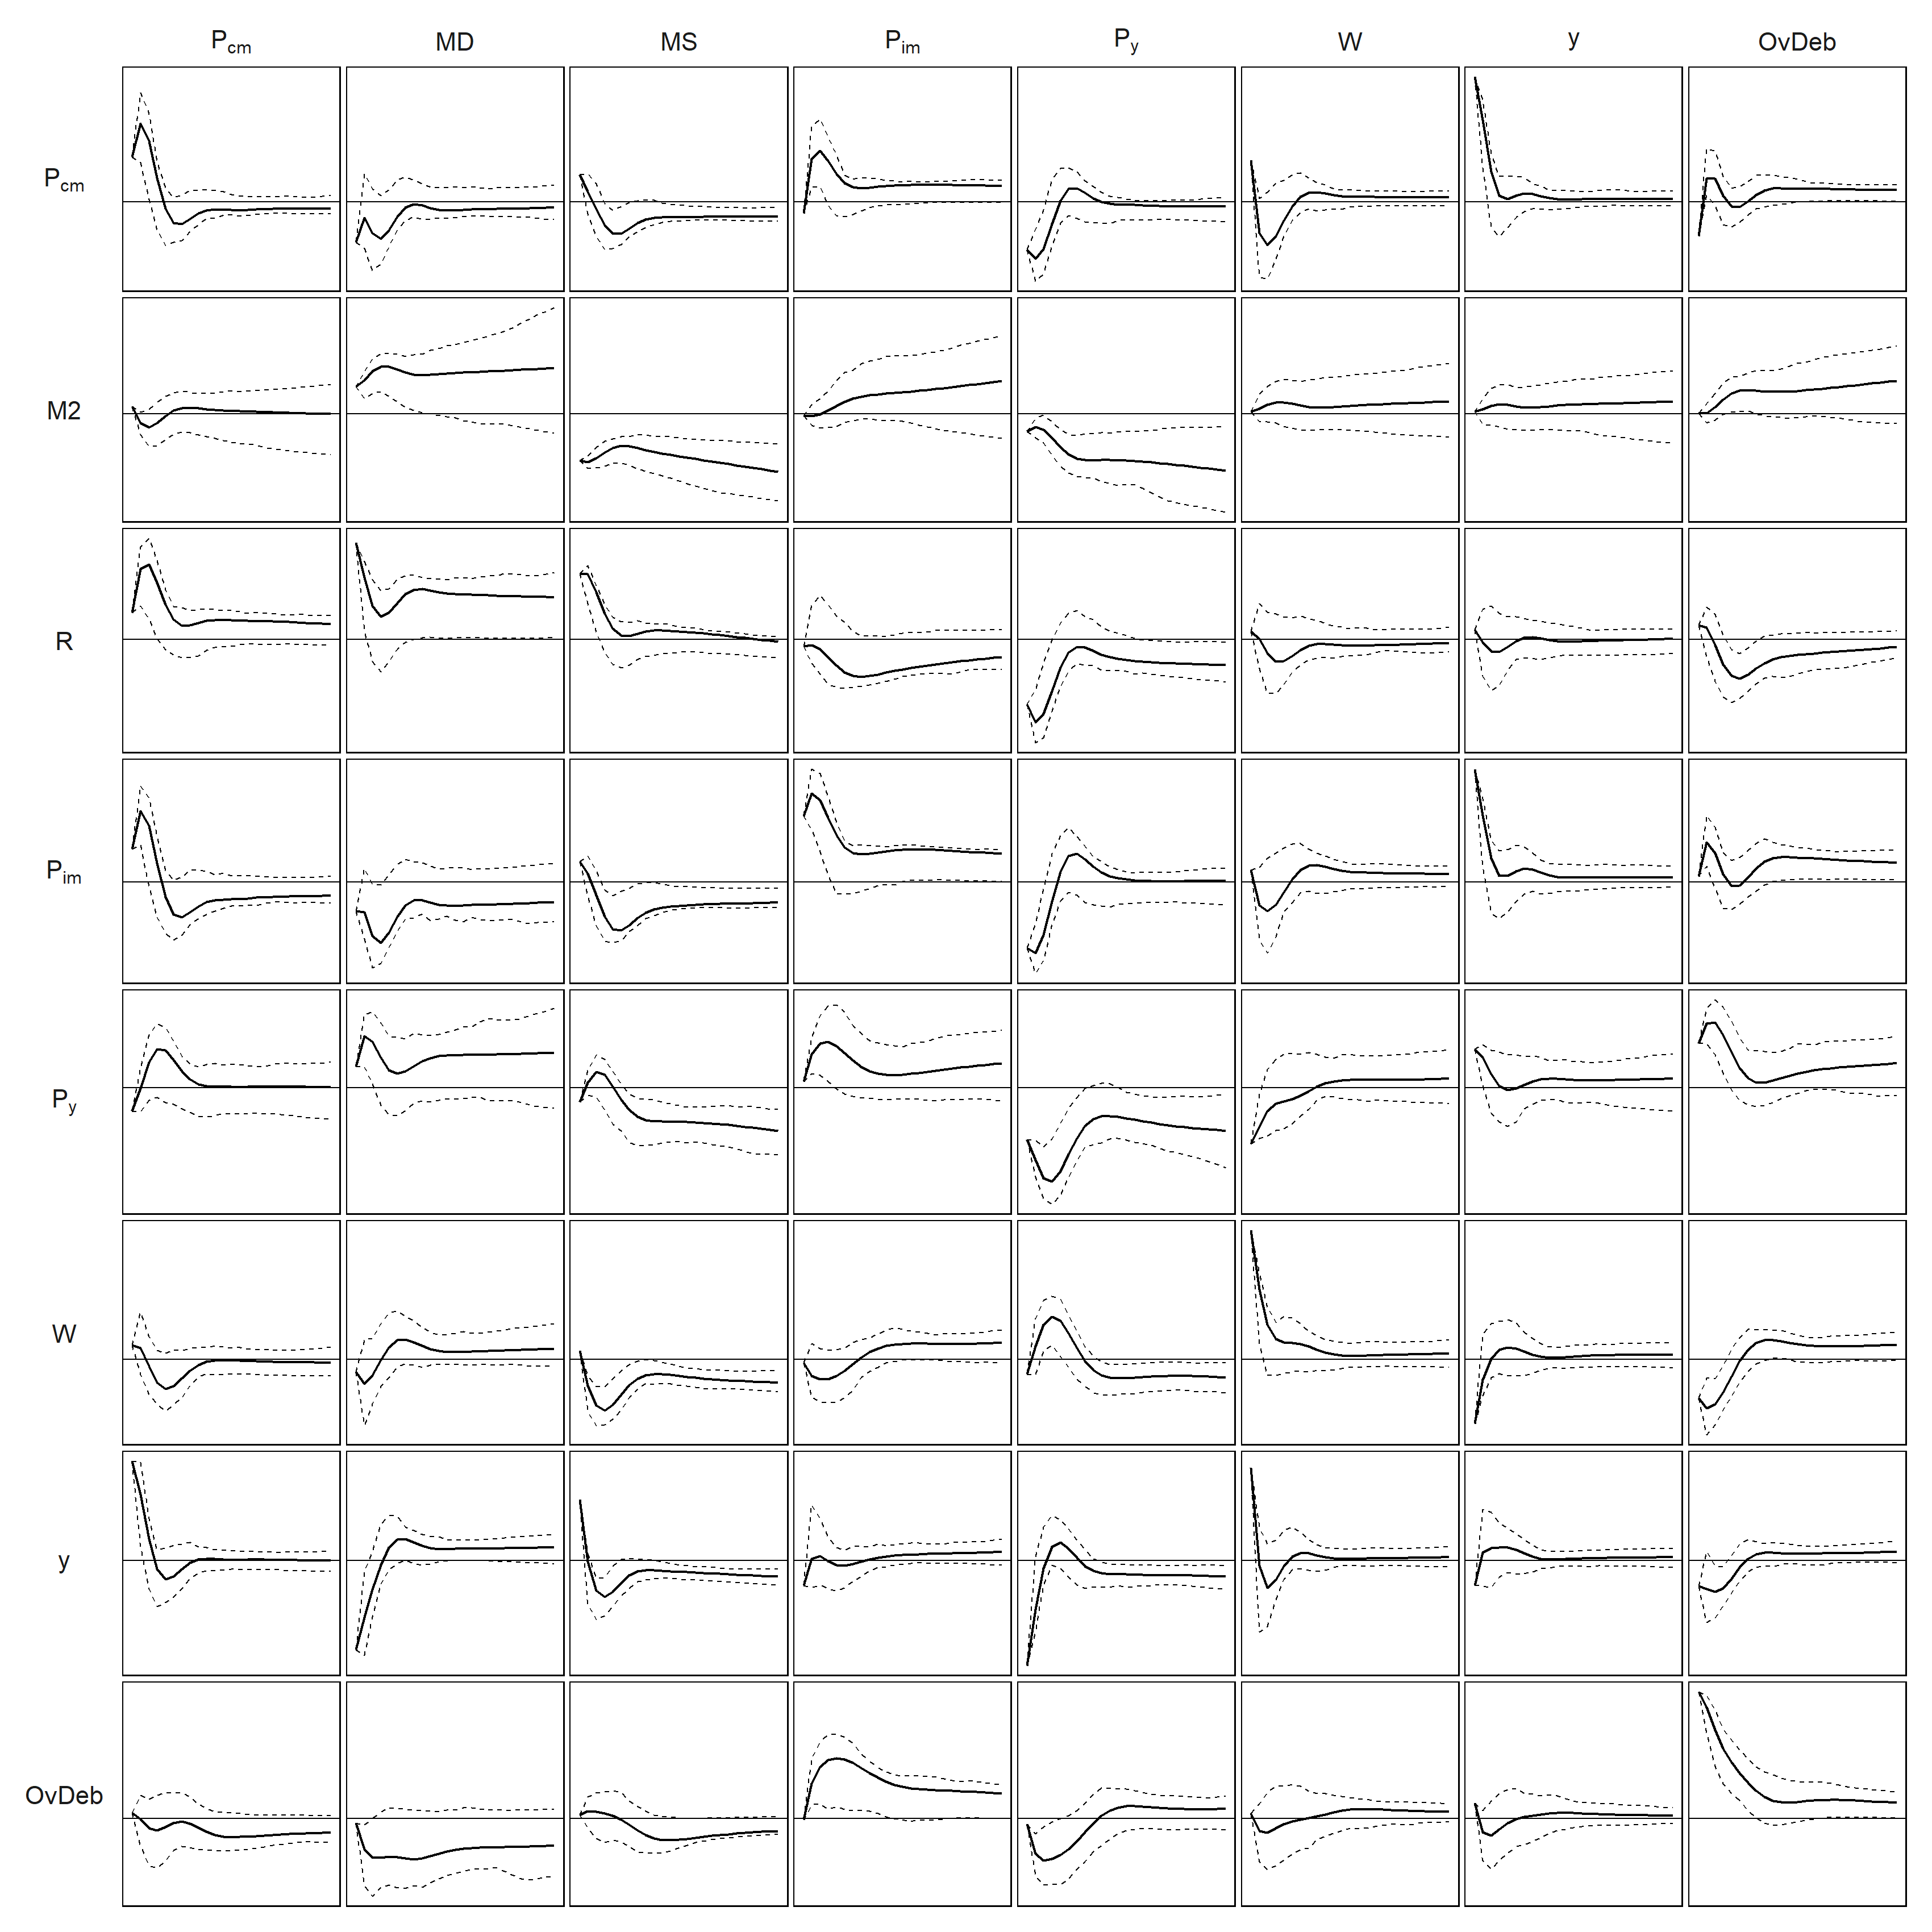
\includegraphics[width=\textwidth]{figures/output/irf_full_grid.png}
    \caption{Функции импульсного отклика для всех структурных шоков}
    \label{fig:irf-full-grid}
\end{figure}
На рисунке \ref{fig:irf-full-grid} показаны функции импульсного отклика для всех структурных шоков. Строки соответствуют реагирующим переменным, столбцы --- источникам шоков. Сплошная линия показывает центральную оценку, пунктирные линии --- интервалы неопределённости. Как и в работе Sims и Zha, этот график используется для проверки того, насколько идентифицированные шоки дают экономически осмысленную динамику.

Основной интерес представляют шоки $MS$ и $MD$. В выбранной нормировке шок $MS$ можно интерпретировать как ужесточение денежно-кредитных условий. После него ставка $R$ резко растёт в первые периоды, а денежный агрегат $M2$ снижается и остаётся ниже начального уровня. Реакция выпуска $y$ имеет краткое начальное повышение, но затем становится отрицательной и постепенно затухает. Уровень цен $P_y$ также после небольшой начальной положительной реакции уходит ниже нуля. В целом это согласуется с базовой логикой денежно-кредитной трансмиссии: рост ставки и сокращение денежной массы сопровождаются снижением выпуска и более слабой динамикой цен.

Шок $MD$ отличается от $MS$. Он сопровождается ростом ставки $R$, положительной реакцией $M2$ и заметным краткосрочным снижением выпуска $y$. Такая динамика ближе к шоку спроса на деньги или ликвидности, а не к самостоятельному ужесточению политики. Реакция $P_y$ на этот шок менее устойчива: в первые периоды она положительна, затем ослабевает, а интервалы неопределённости остаются широкими, что может объясняться лагами денежно-кредитной политики.

Шоки $P_{cm}$, $P_{im}$, $P_y$, выпуска и просроченной задолженности $OvDeb$ дают заметные реакции цен, выпуска и ставки. Особенно важно, что неденежные шоки также вызывают движение $R$ и $M2$, то есть денежно-кредитные переменные реагируют на состояние экономики. Поэтому по функциям импульсного отклика нельзя делать вывод о роли политики в кризисах. Для этого требуется историческая декомпозиция и анализ структурных шоков.

\subsection{Историческая декомпозиция и структурные шоки}
На рисунках \ref{fig:hd-m2}--\ref{fig:hd-gdp} показана историческая декомпозиция прогнозных ошибок для четырёх основных переменных: денежного агрегата $M2$, ставки $R$, уровня цен $P_y$ и выпуска $y$. Верхняя панель каждого графика показывает общую прогнозную ошибку, остальные панели --- вклад отдельных структурных шоков. Заштрихованные области соответствуют эпизодам 2014--2015, 2020 и 2022 годов.

\begin{figure}[!htbp]
    \centering
    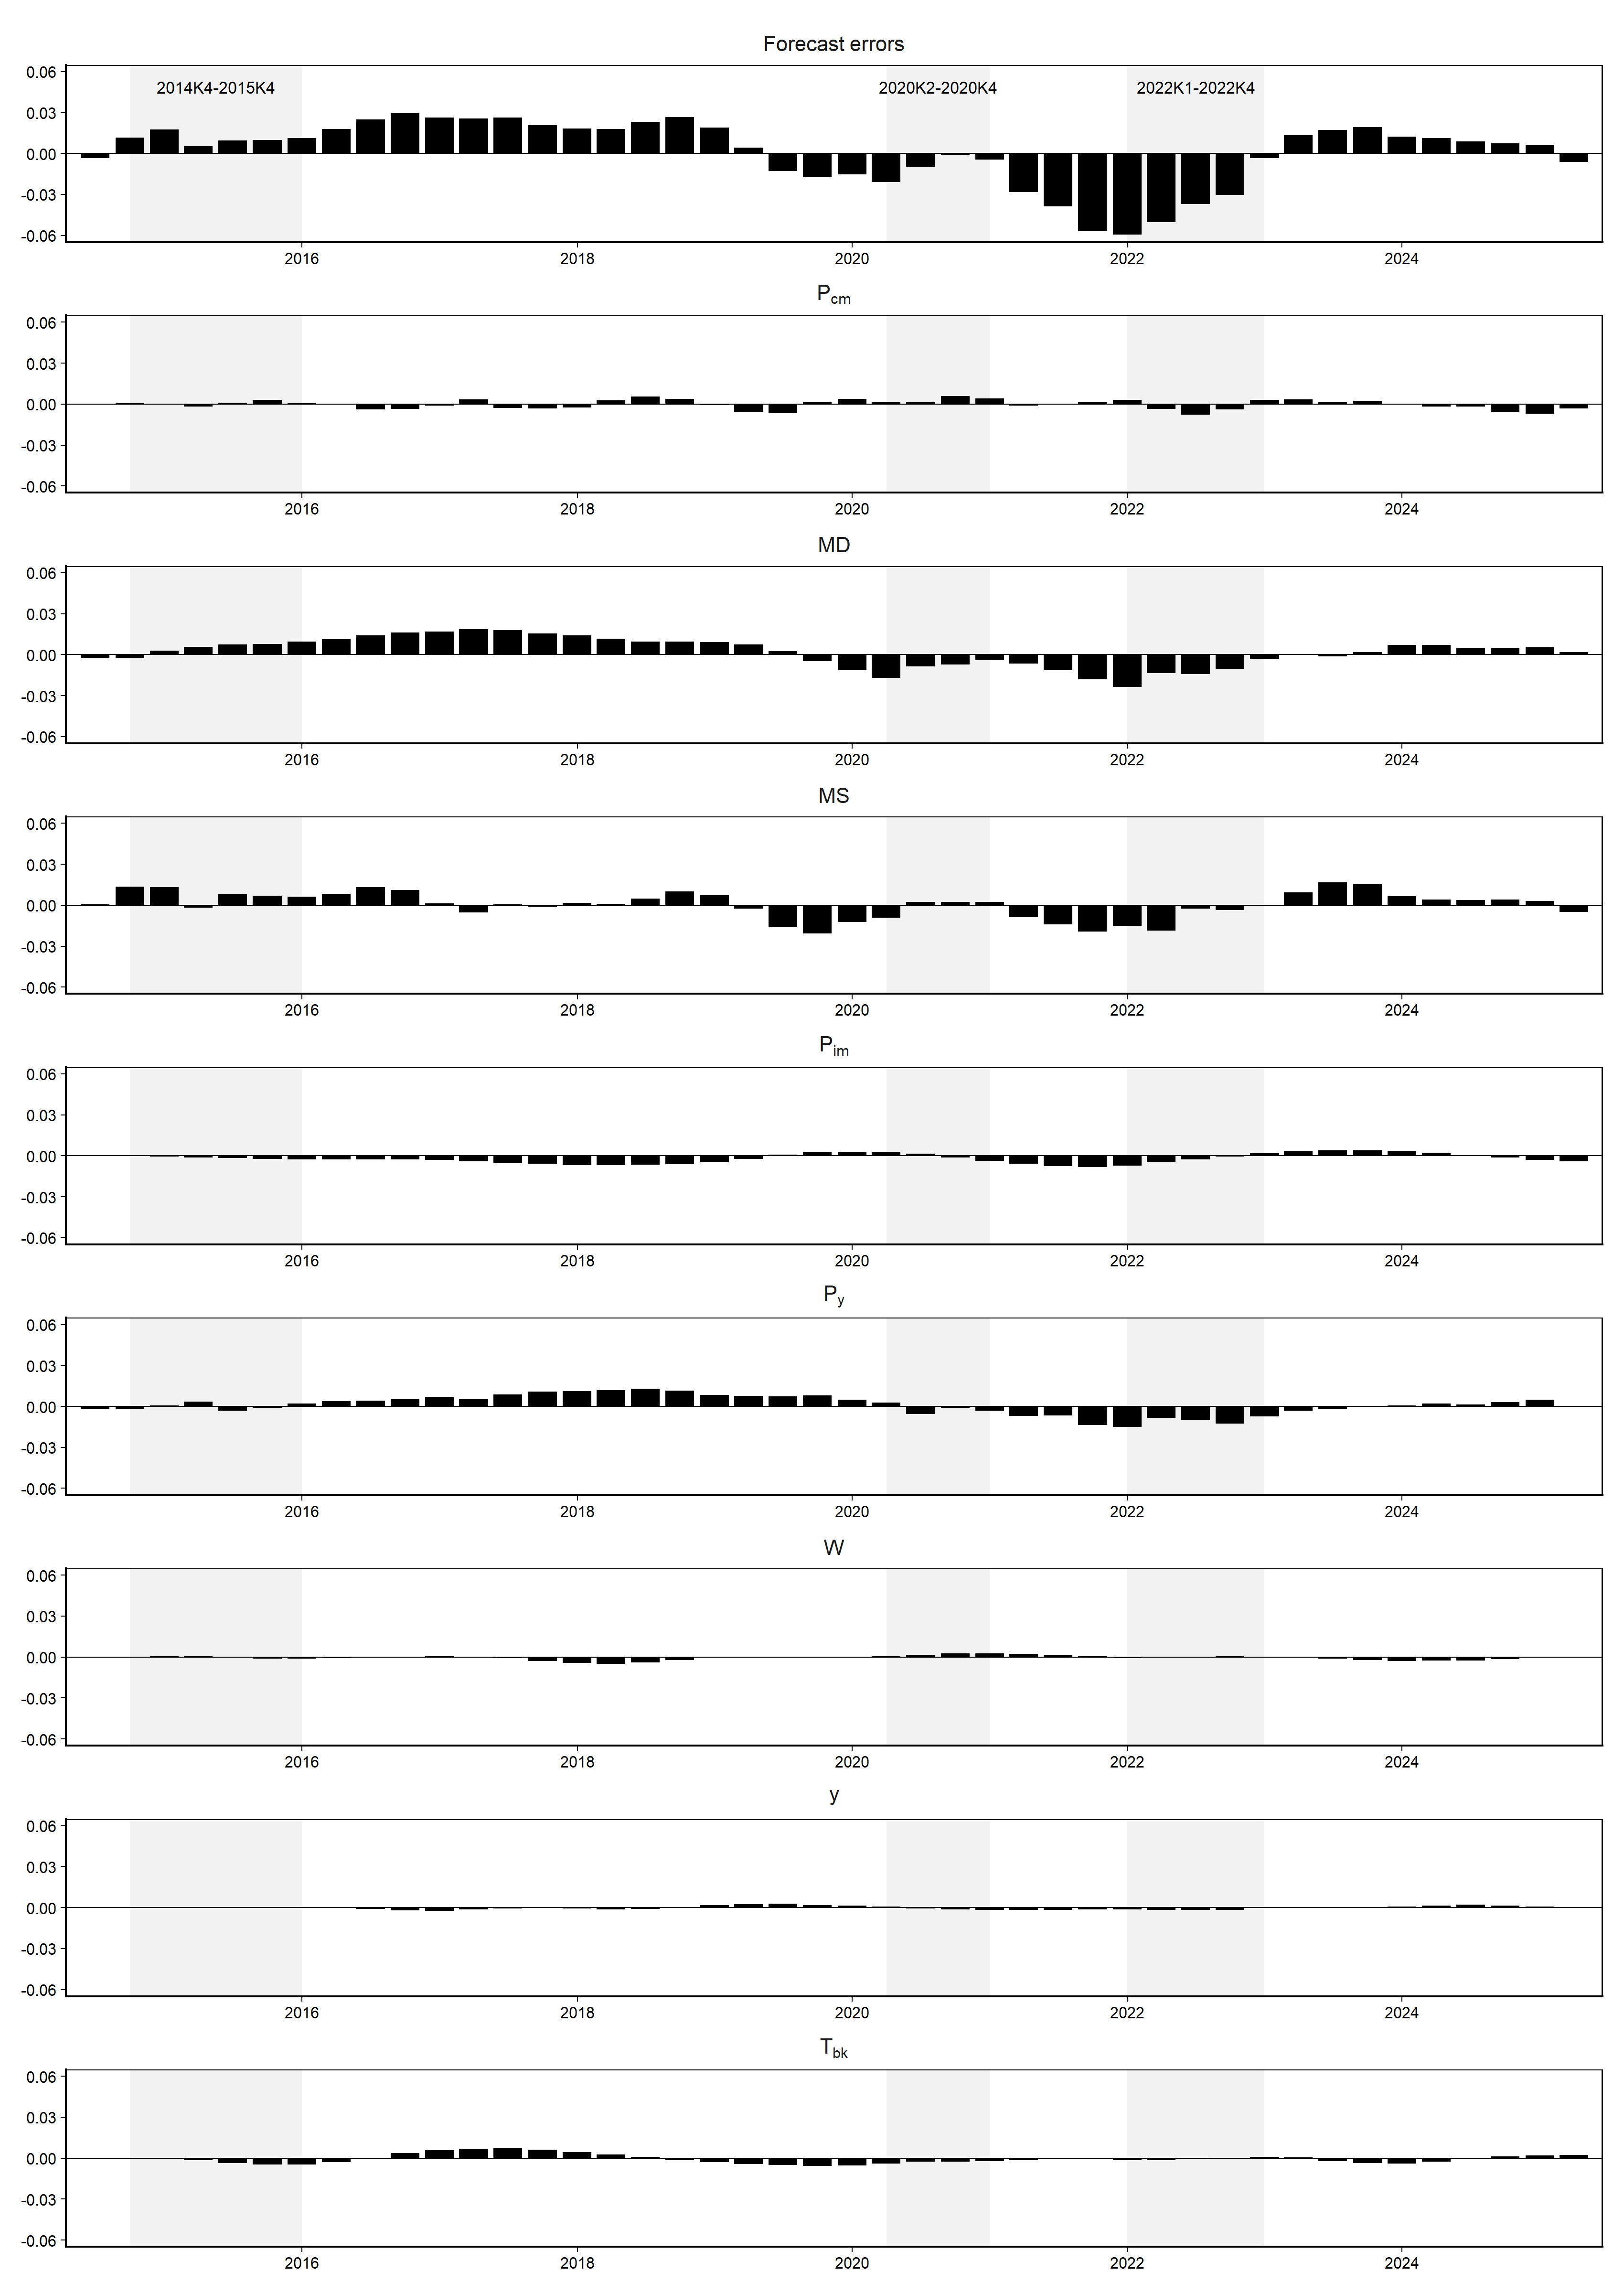
\includegraphics[width=\textwidth]{figures/output/historical_decomposition_m2.png}
    \caption{Историческая декомпозиция прогнозных ошибок для $M2$}
    \label{fig:hd-m2}
\end{figure}
Для $M2$ декомпозиция показывает (рис. \ref{fig:hd-m2}), что отклонения денежного агрегата не сводятся к шоку $MS$. В 2021--2022 годах отрицательная прогнозная ошибка $M2$ связана сразу с несколькими компонентами: $MS$, $MD$, $P_y$ и $P_{im}$. Поэтому снижение денежного агрегата в этот период лучше трактовать не как чистый денежно-кредитный шок, а как результат совместного действия политики, спроса на деньги и ценовых шоков.

\begin{figure}[!htbp]
    \centering
    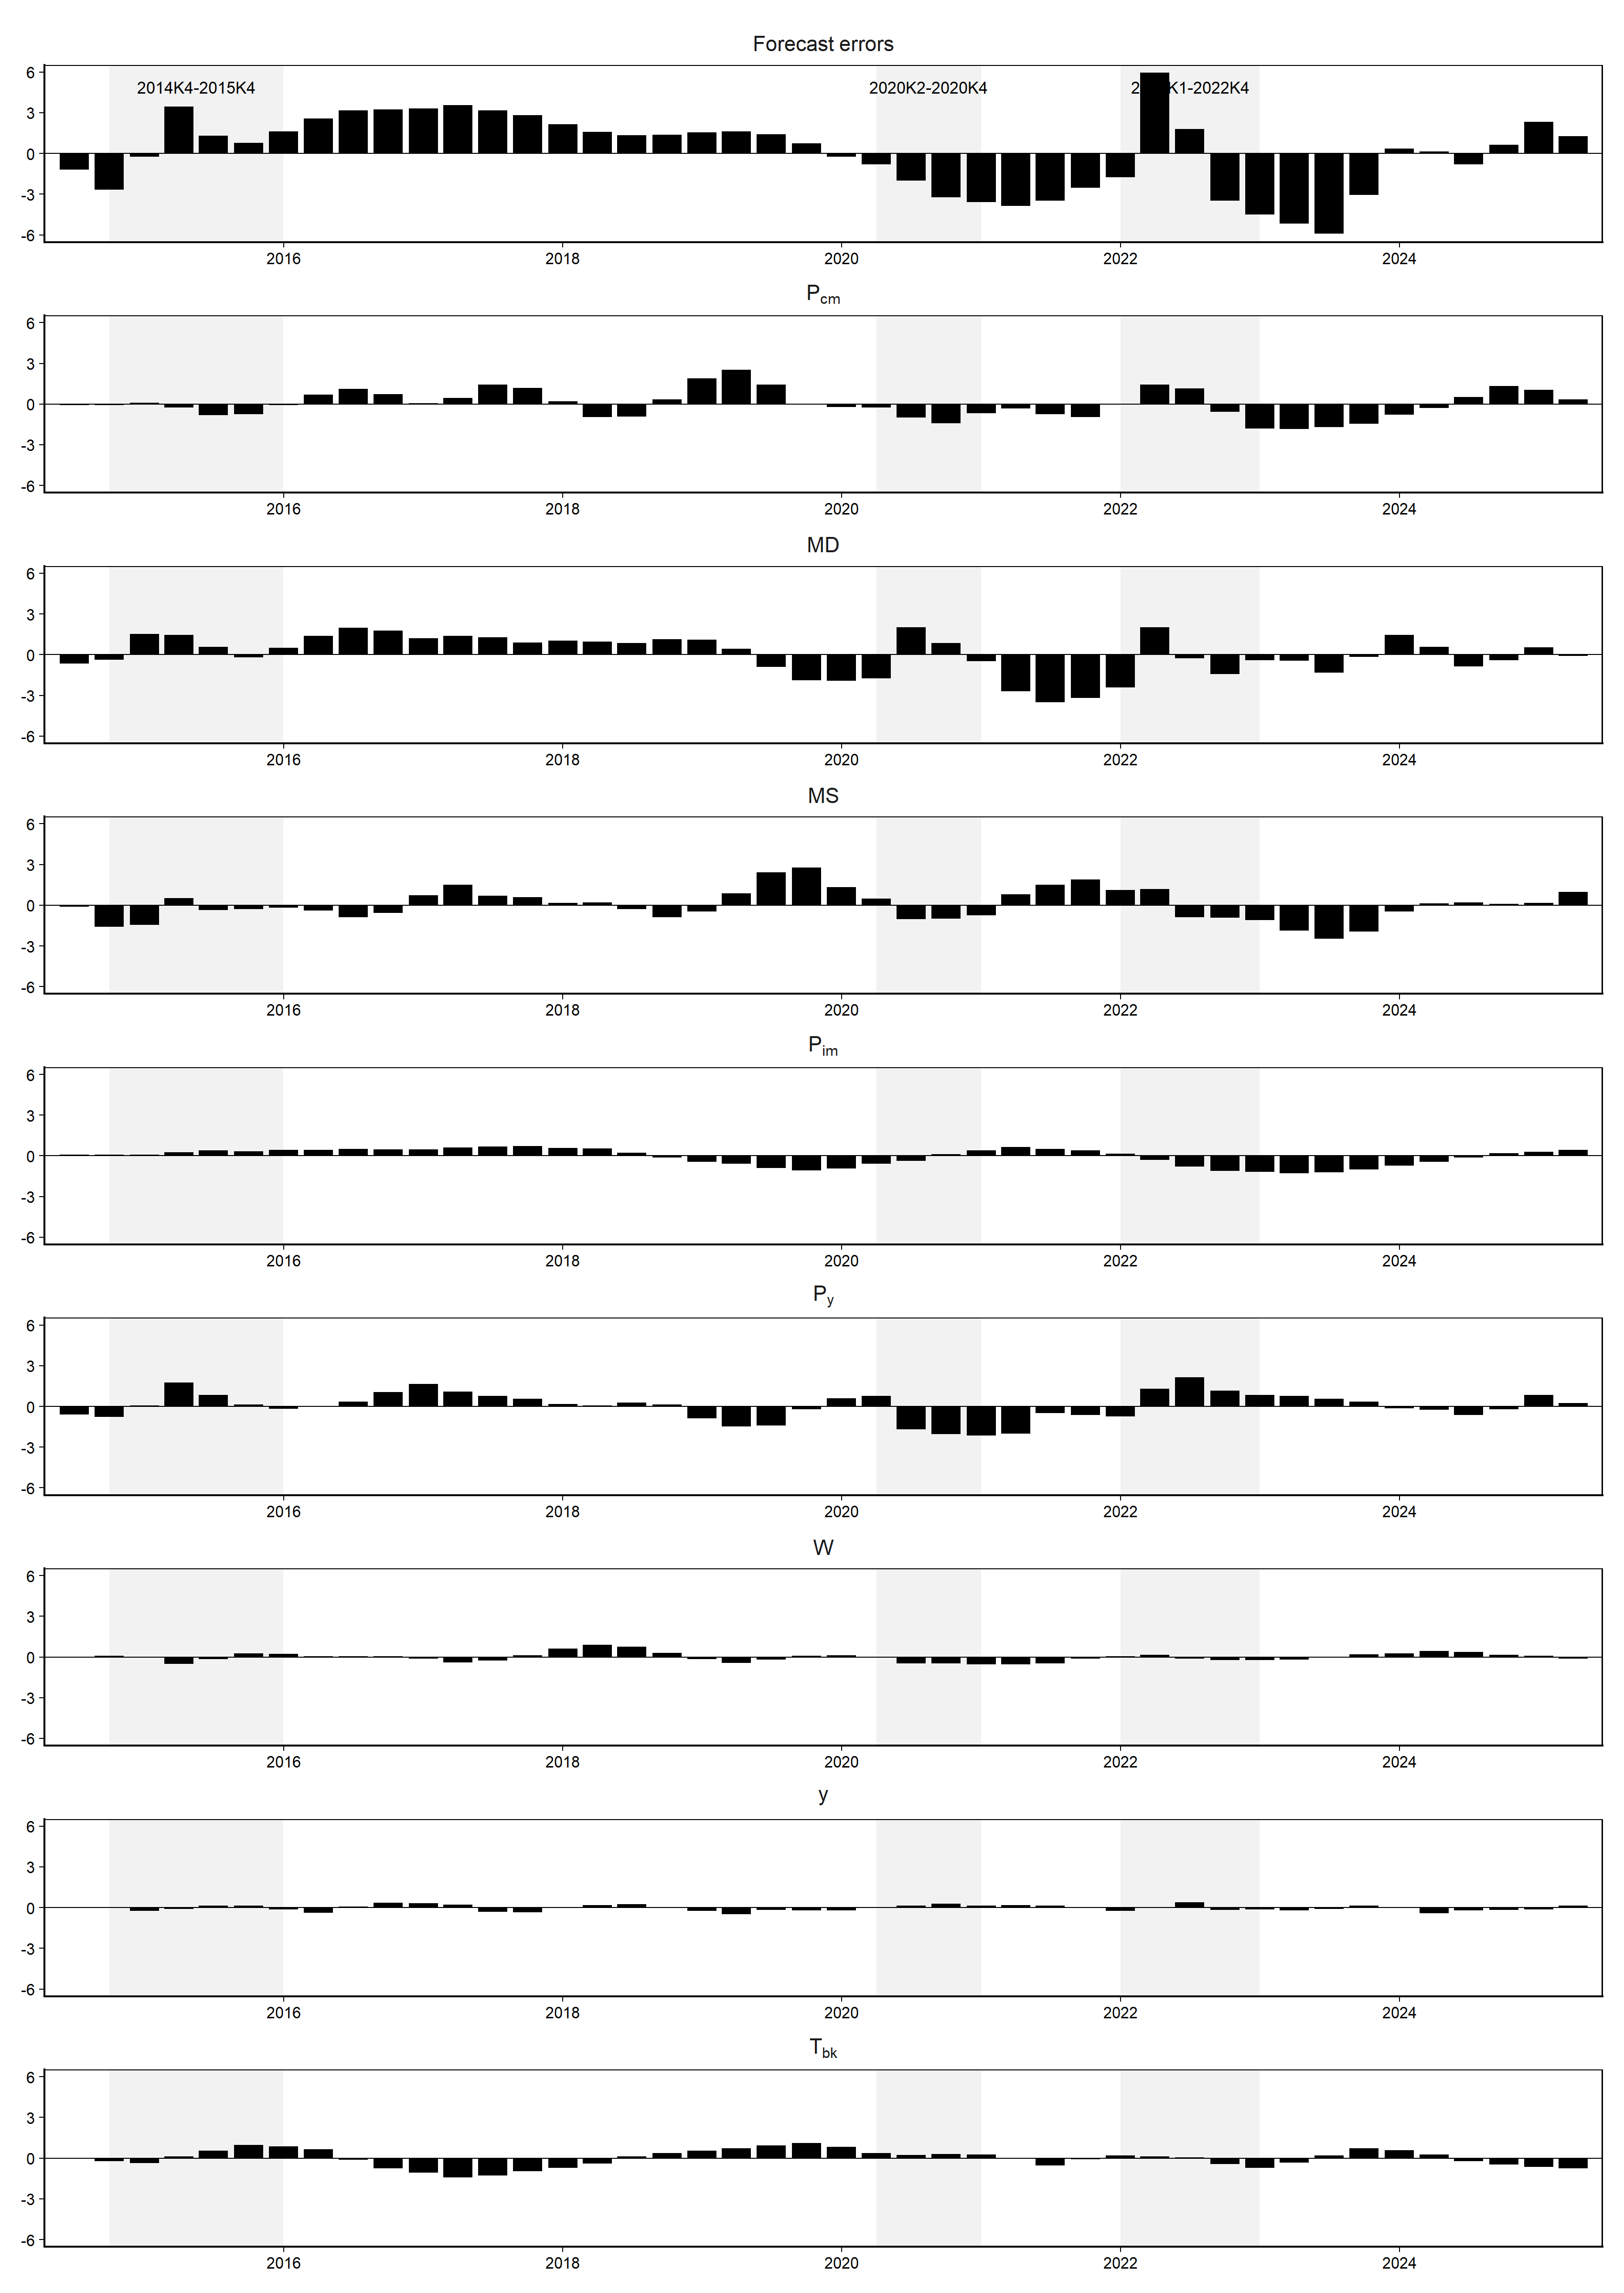
\includegraphics[width=\textwidth]{figures/output/historical_decomposition_key_rate.png}
    \caption{Историческая декомпозиция прогнозных ошибок для $R$}
    \label{fig:hd-key-rate}
\end{figure}
Для ставки $R$ картина (рис. \ref{fig:hd-key-rate}) также не сводится к одному шоку $MS$. В 2015--2017 годах положительная прогнозная ошибка ставки поддерживается несколькими компонентами, включая $MD$, $P_y$, $P_{cm}$ и $OvDeb$. В 2022 году резкий положительный вклад в ставку дают не только $MS$, но и шоки денежного спроса и ценовые шоки. Это согласуется с логикой Sims и Zha: движение ставки отражает не только самостоятельные сдвиги политики, но и систематическую реакцию на состояние экономики.

\begin{figure}[!htbp]
    \centering
    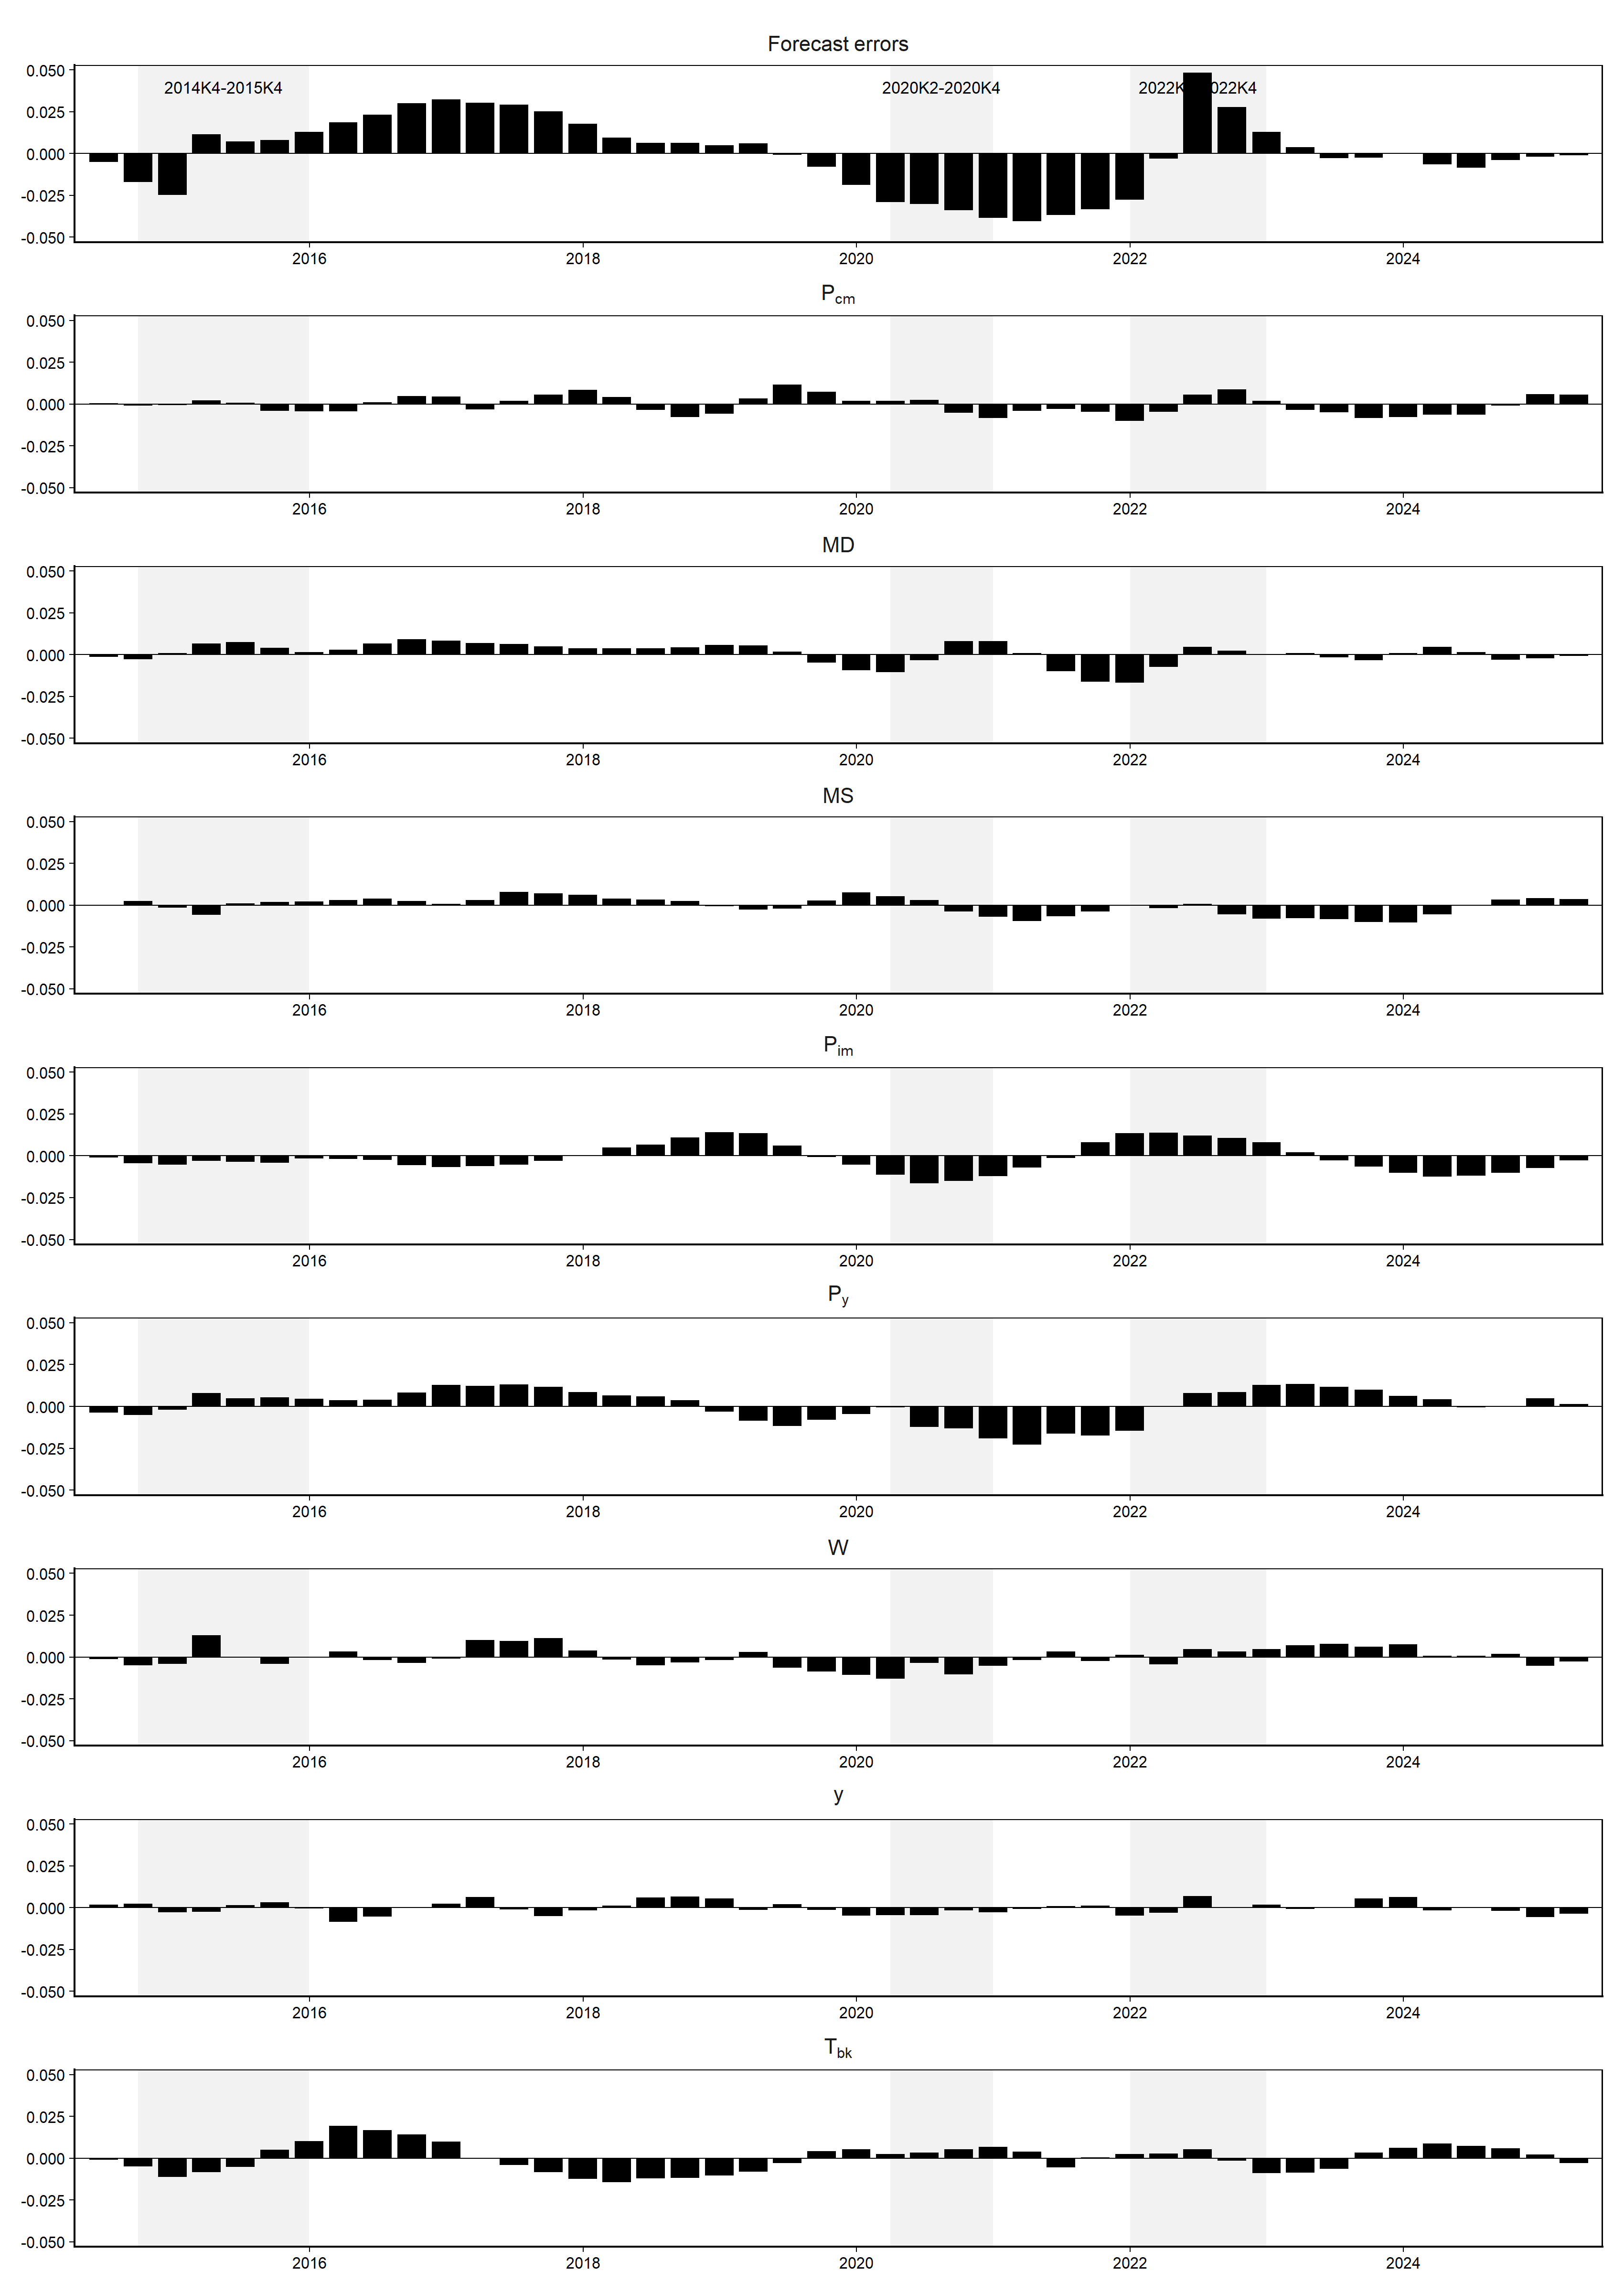
\includegraphics[width=\textwidth]{figures/output/historical_decomposition_cpi.png}
    \caption{Историческая декомпозиция прогнозных ошибок для $P_y$}
    \label{fig:hd-cpi}
\end{figure}
Для $P_y$ (рис. \ref{fig:hd-cpi}) основной результат состоит в том, что ценовая динамика заметно связана с неденежными шоками. В 2020 году отрицательная прогнозная ошибка уровня цен в основном поддерживается компонентами $P_y$, $P_{im}$, $P_{cm}$ и $MS$. В 2022 году положительная ошибка уровня цен объясняется прежде всего ценовыми шоками и шоками со стороны экономики, тогда как вклад $MS$ не является главным. Поэтому ускорение цен в модели не следует напрямую приписывать только денежно-кредитной политике.

\begin{figure}[!htbp]
    \centering
    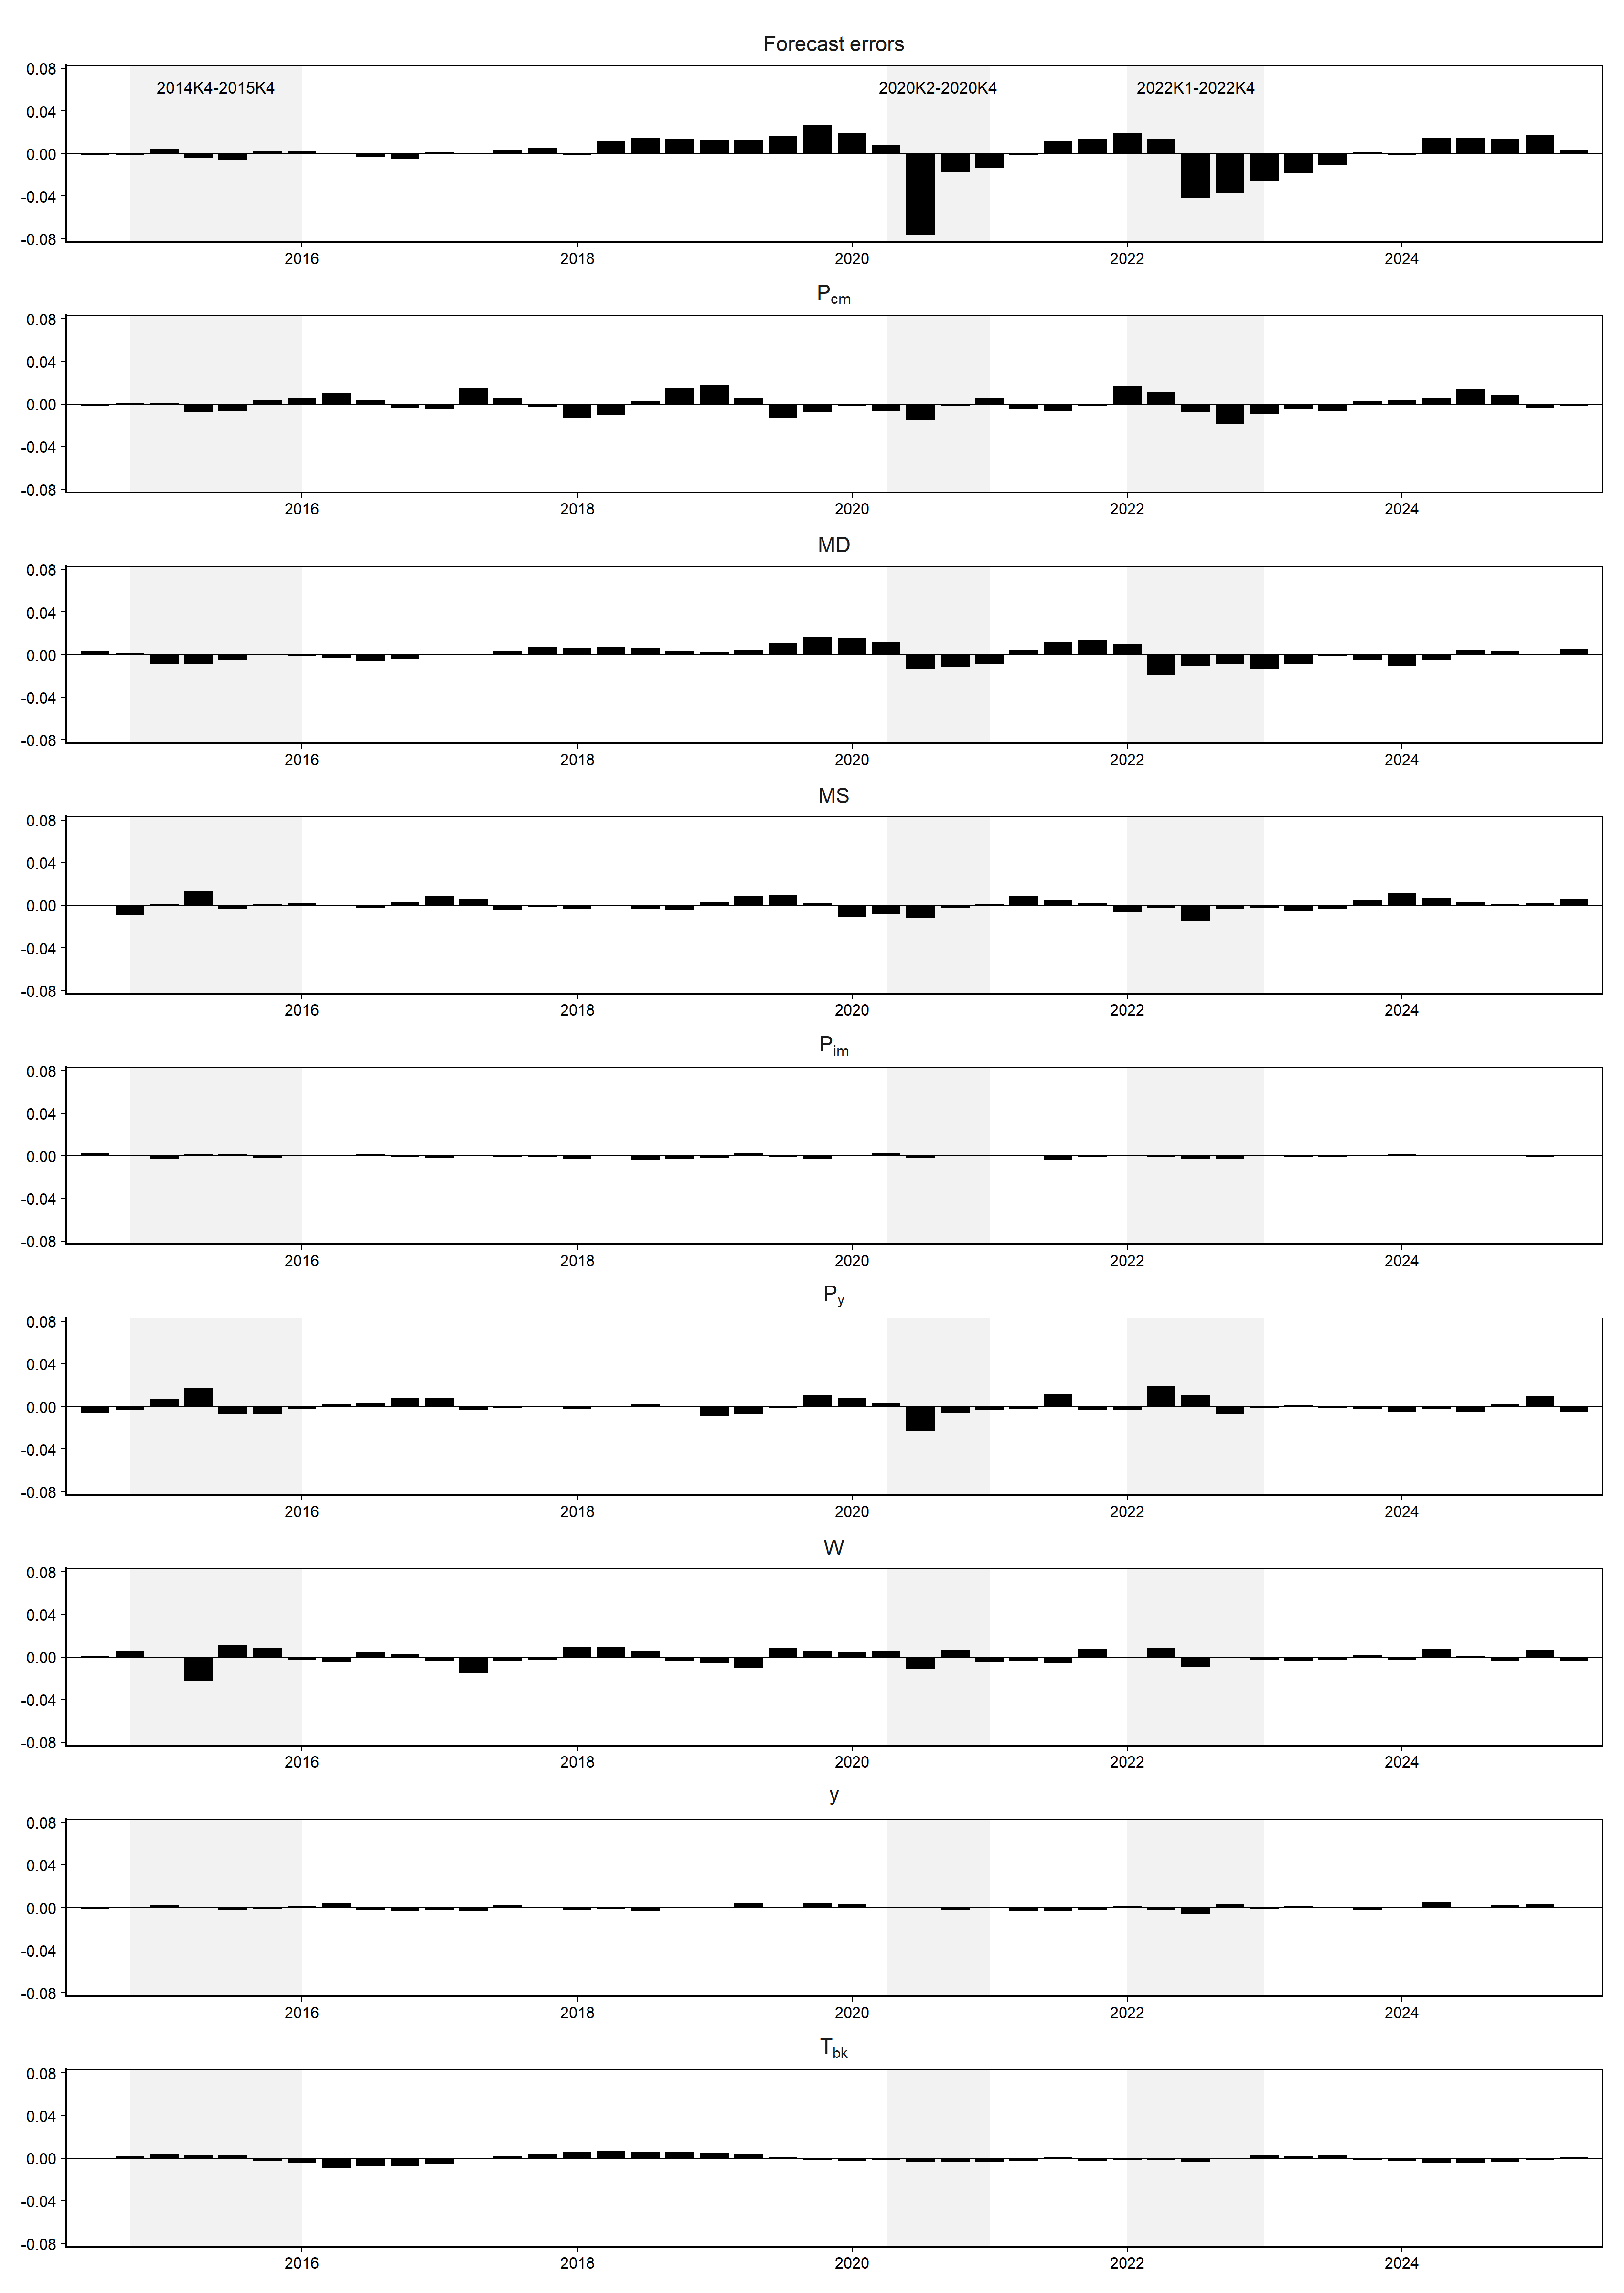
\includegraphics[width=\textwidth]{figures/output/historical_decomposition_gdp.png}
    \caption{Историческая декомпозиция прогнозных ошибок для $y$}
    \label{fig:hd-gdp}
\end{figure}
Для выпуска $y$ (рис. \ref{fig:hd-gdp}) денежно-кредитные шоки имеют заметный, но не доминирующий вклад. В 2020 году отрицательная прогнозная ошибка выпуска связана с несколькими компонентами: $P_y$, $P_{cm}$, $MD$ и $MS$. В 2022 году отрицательный вклад $MS$ также присутствует, но рядом с ним остаются вклады $MD$, $P_{cm}$, $W$, $P_{im}$ и других шоков. Это означает, что спад выпуска в декомпозиции не объясняется одним денежно-кредитным шоком.

Таким образом, историческая декомпозиция уточняет выводы из функций импульсного отклика. Шок $MS$ в модели имеет экономически осмысленную динамику и может снижать выпуск, однако вклад денежно-кредитных шоков в кризисные эпизоды не является единственным. Существенная часть движения $M2$, $R$, $P_y$ и $y$ связана с неденежными шоками и реакцией политики на состояние экономики.

\begin{figure}[!htbp]
    \centering
    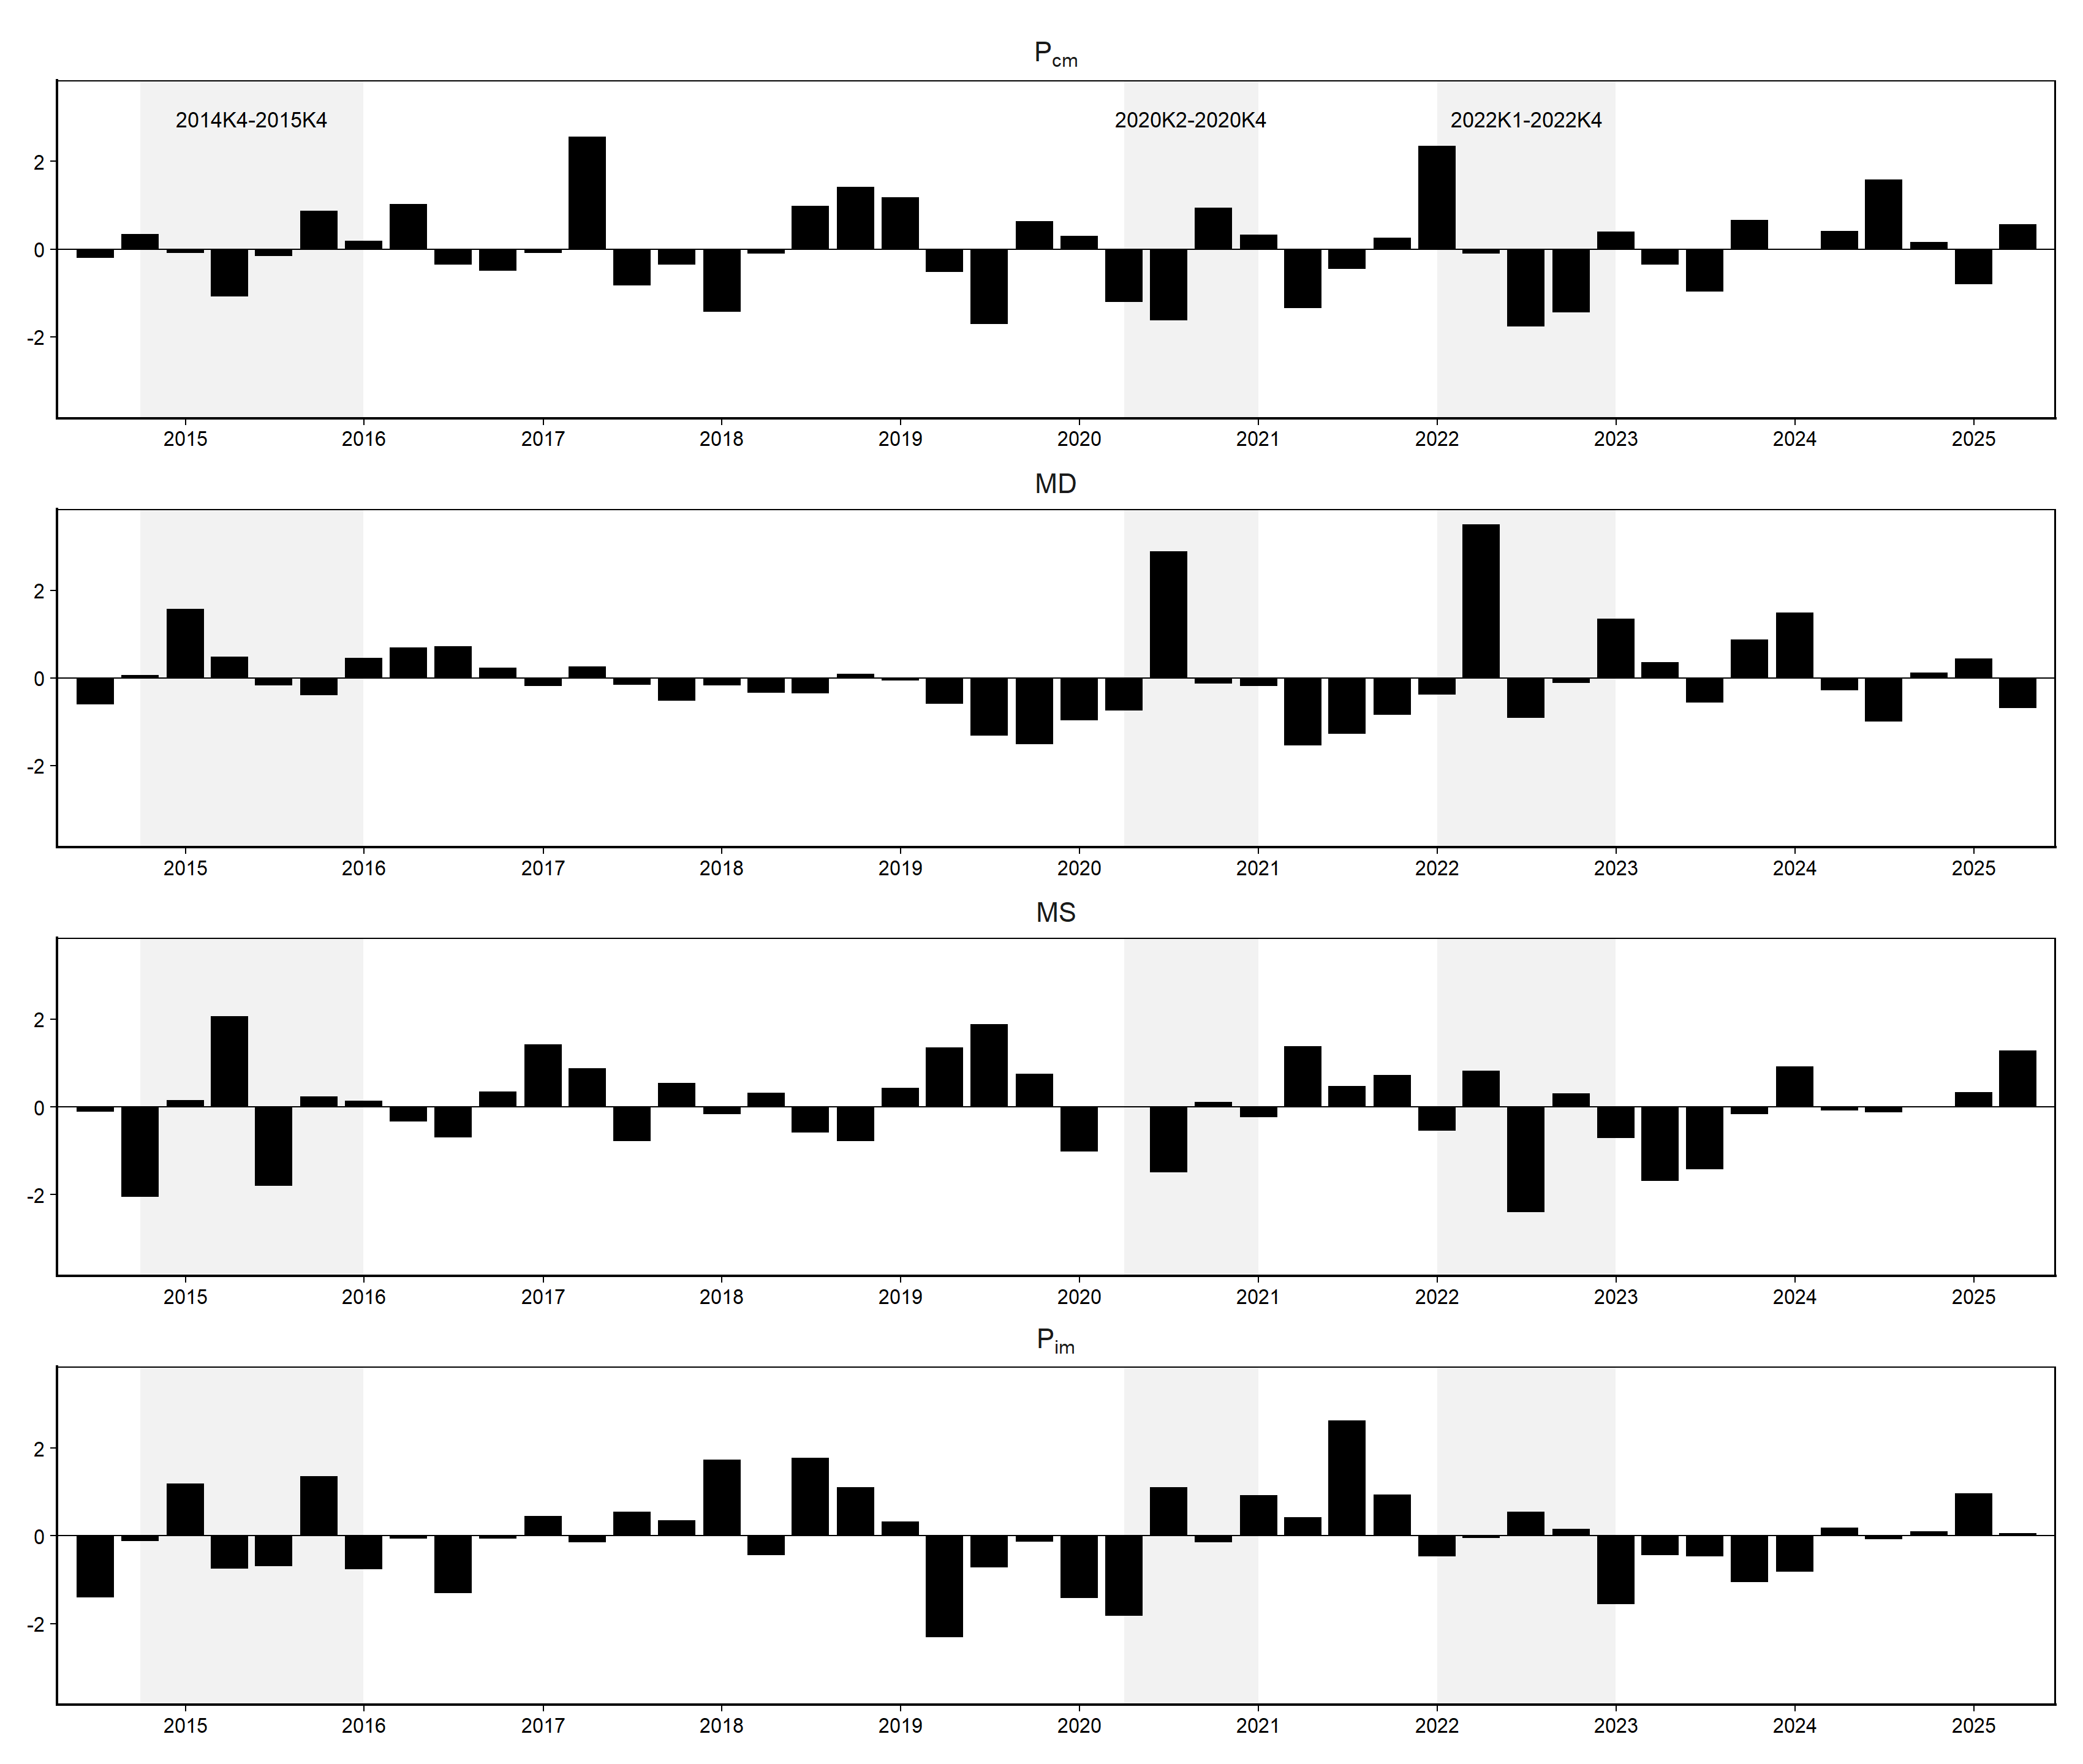
\includegraphics[width=\textwidth]{figures/output/structural_shocks_8a.png}
    \caption{Структурные шоки: первая группа}
    \label{fig:structural-shocks-8a}
\end{figure}

\begin{figure}[!htbp]
    \centering
    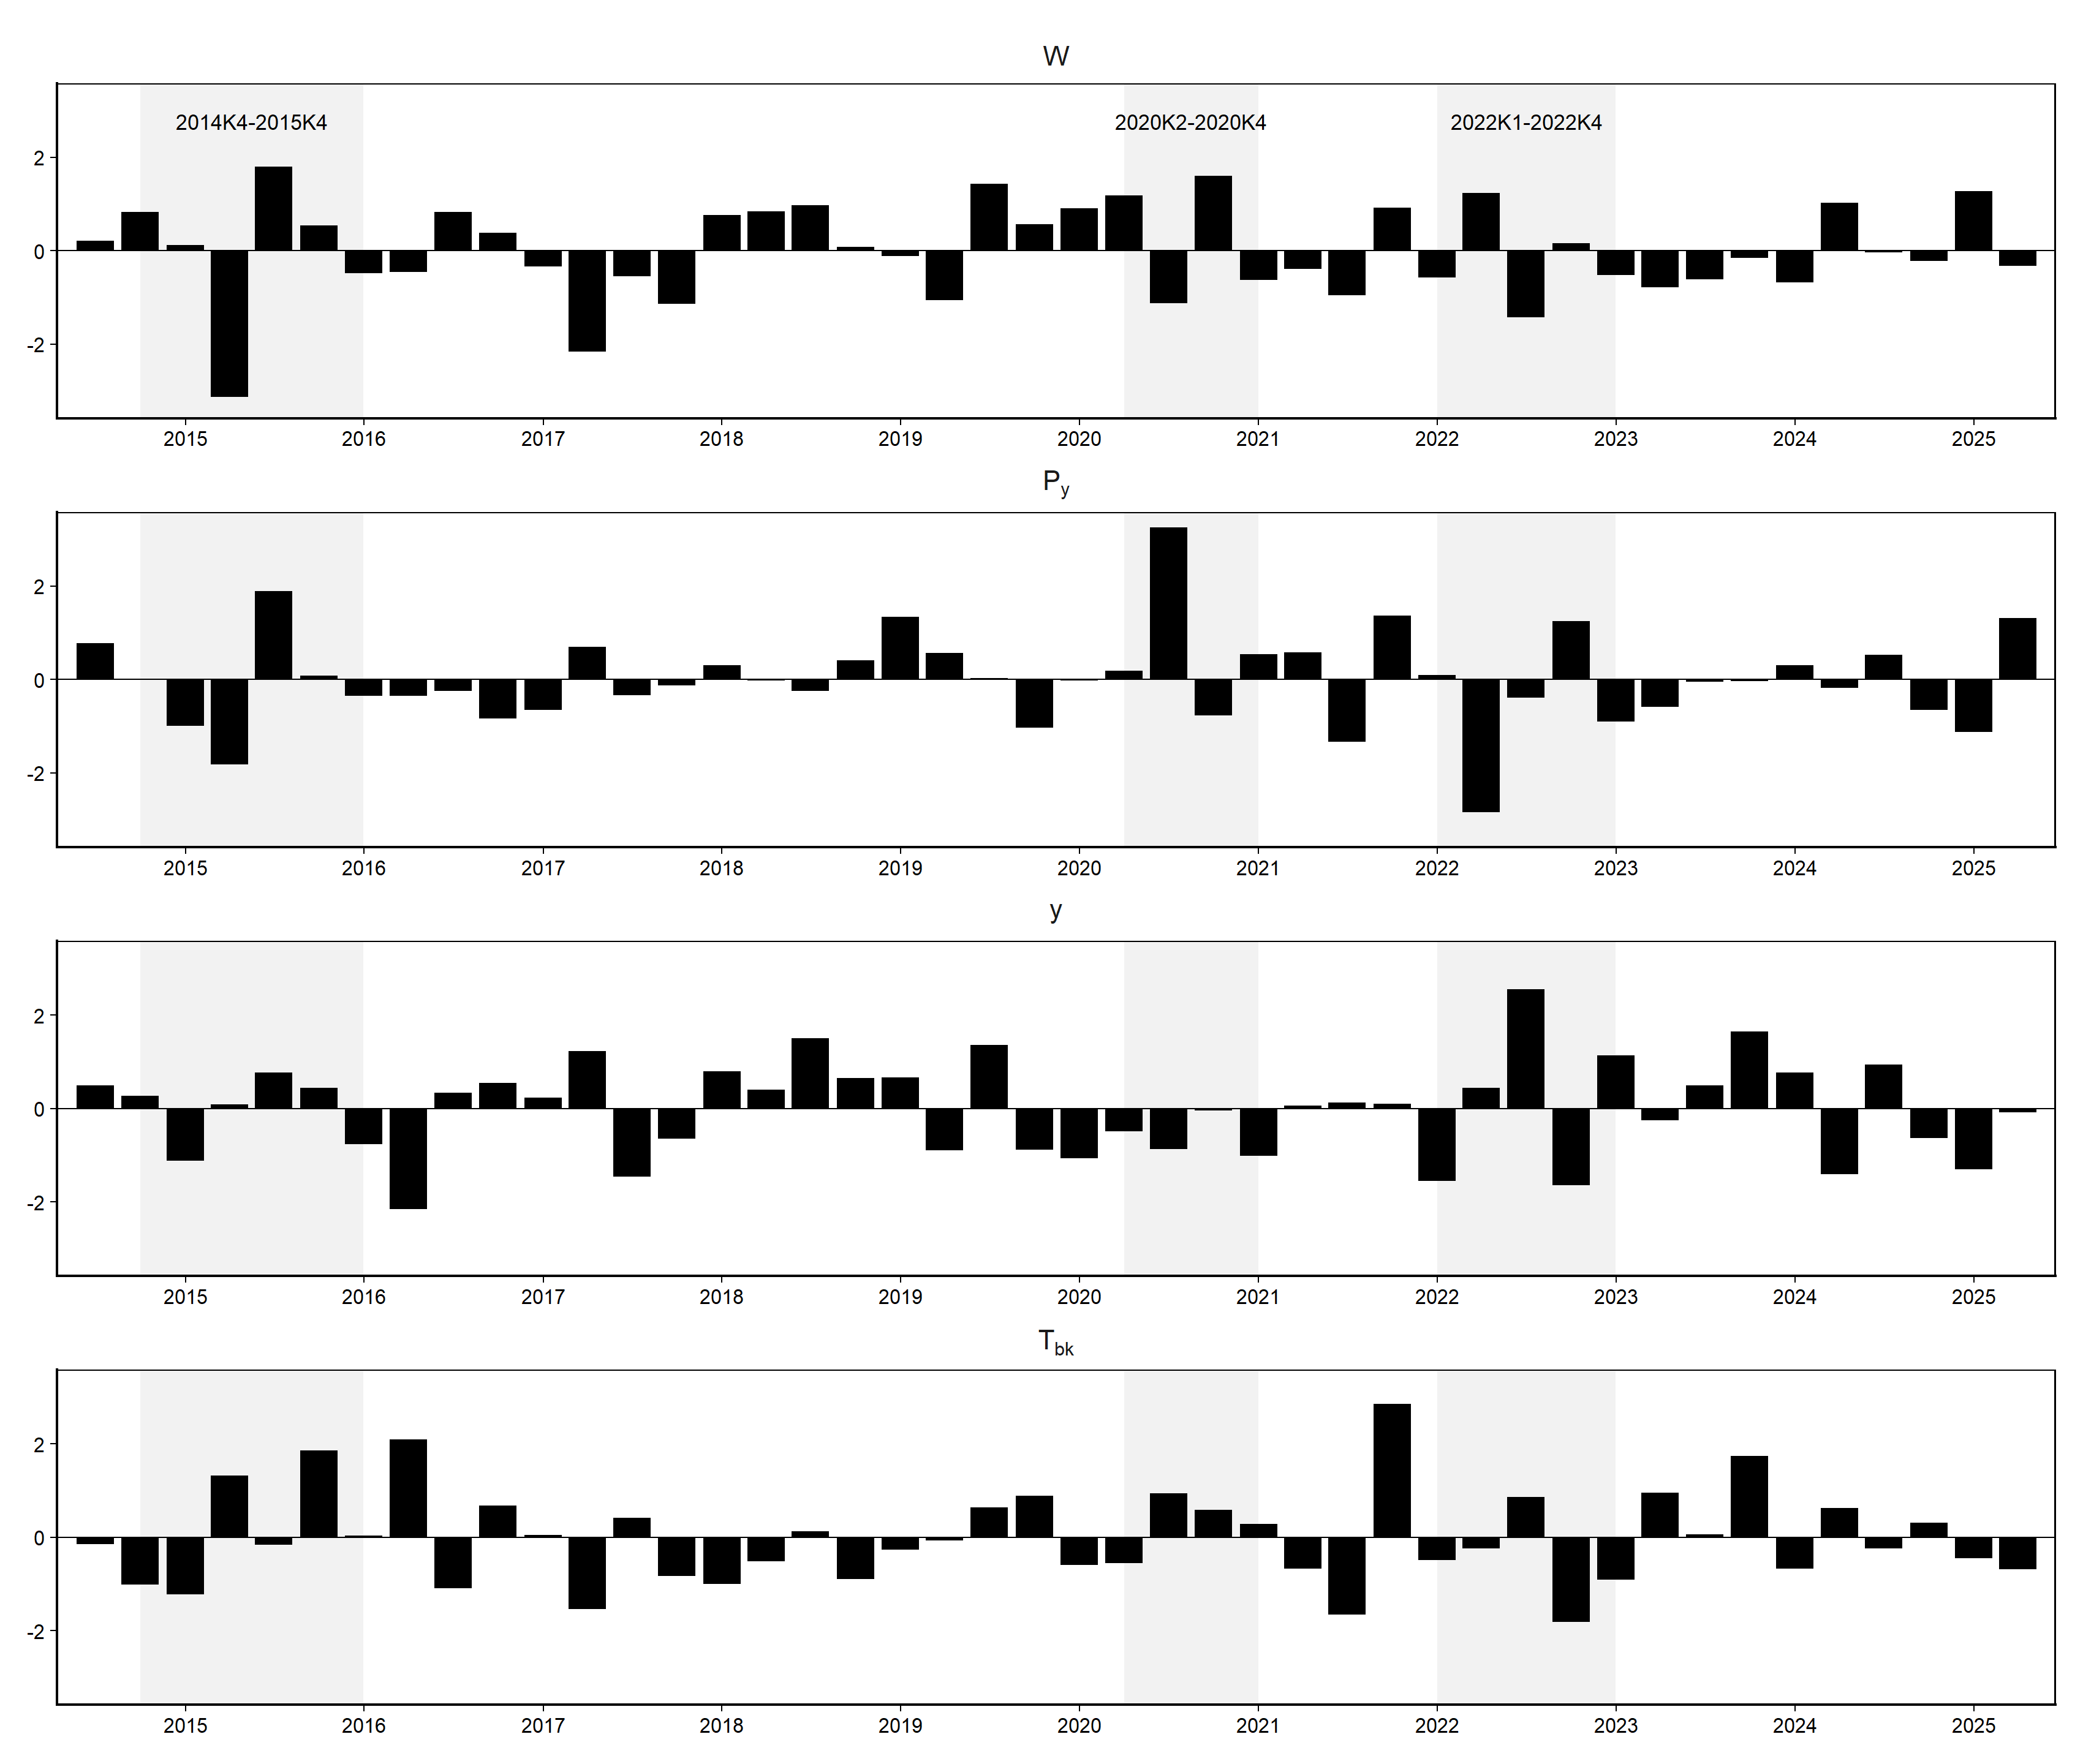
\includegraphics[width=\textwidth]{figures/output/structural_shocks_8b.png}
    \caption{Структурные шоки: вторая группа}
    \label{fig:structural-shocks-8b}
\end{figure}

На рисунках \ref{fig:structural-shocks-8a}--\ref{fig:structural-shocks-8b} показаны временные ряды структурных шоков. Эти графики дополняют историческую декомпозицию: они позволяют проверить, какие неожиданные шоки приходятся на кризисные эпизоды 2014--2015, 2020 и 2022 годов.

Шок $MS$ заметен в отдельные кварталы, но не является единственным крупным шоком в выделенные периоды. В 2014--2015 годах рядом с ним видны колебания $MD$, $P_{cm}$ и $P_{im}$. В 2020 году сильнее выделяются $MD$, $P_y$ и реальные шоки. В 2022 году $MS$ также присутствует, но одновременно наблюдаются крупные шоки $MD$, $P_{cm}$, $P_{im}$, $W$, $y$ и $OvDeb$.

Поэтому ряды структурных шоков подтверждают вывод исторической декомпозиции: кризисные эпизоды не сводятся к автономным шокам денежно-кредитной политики. Движение ставки, денежного агрегата, цен и выпуска лучше интерпретировать как результат сочетания нескольких шоков и реакции политики на состояние экономики.


\subsection[Контрфактическая политика: фиксированные M2 и R]{Контрфактическая политика: фиксированные $M2$ и $R$}

\begin{figure}[!htbp]
    \centering
    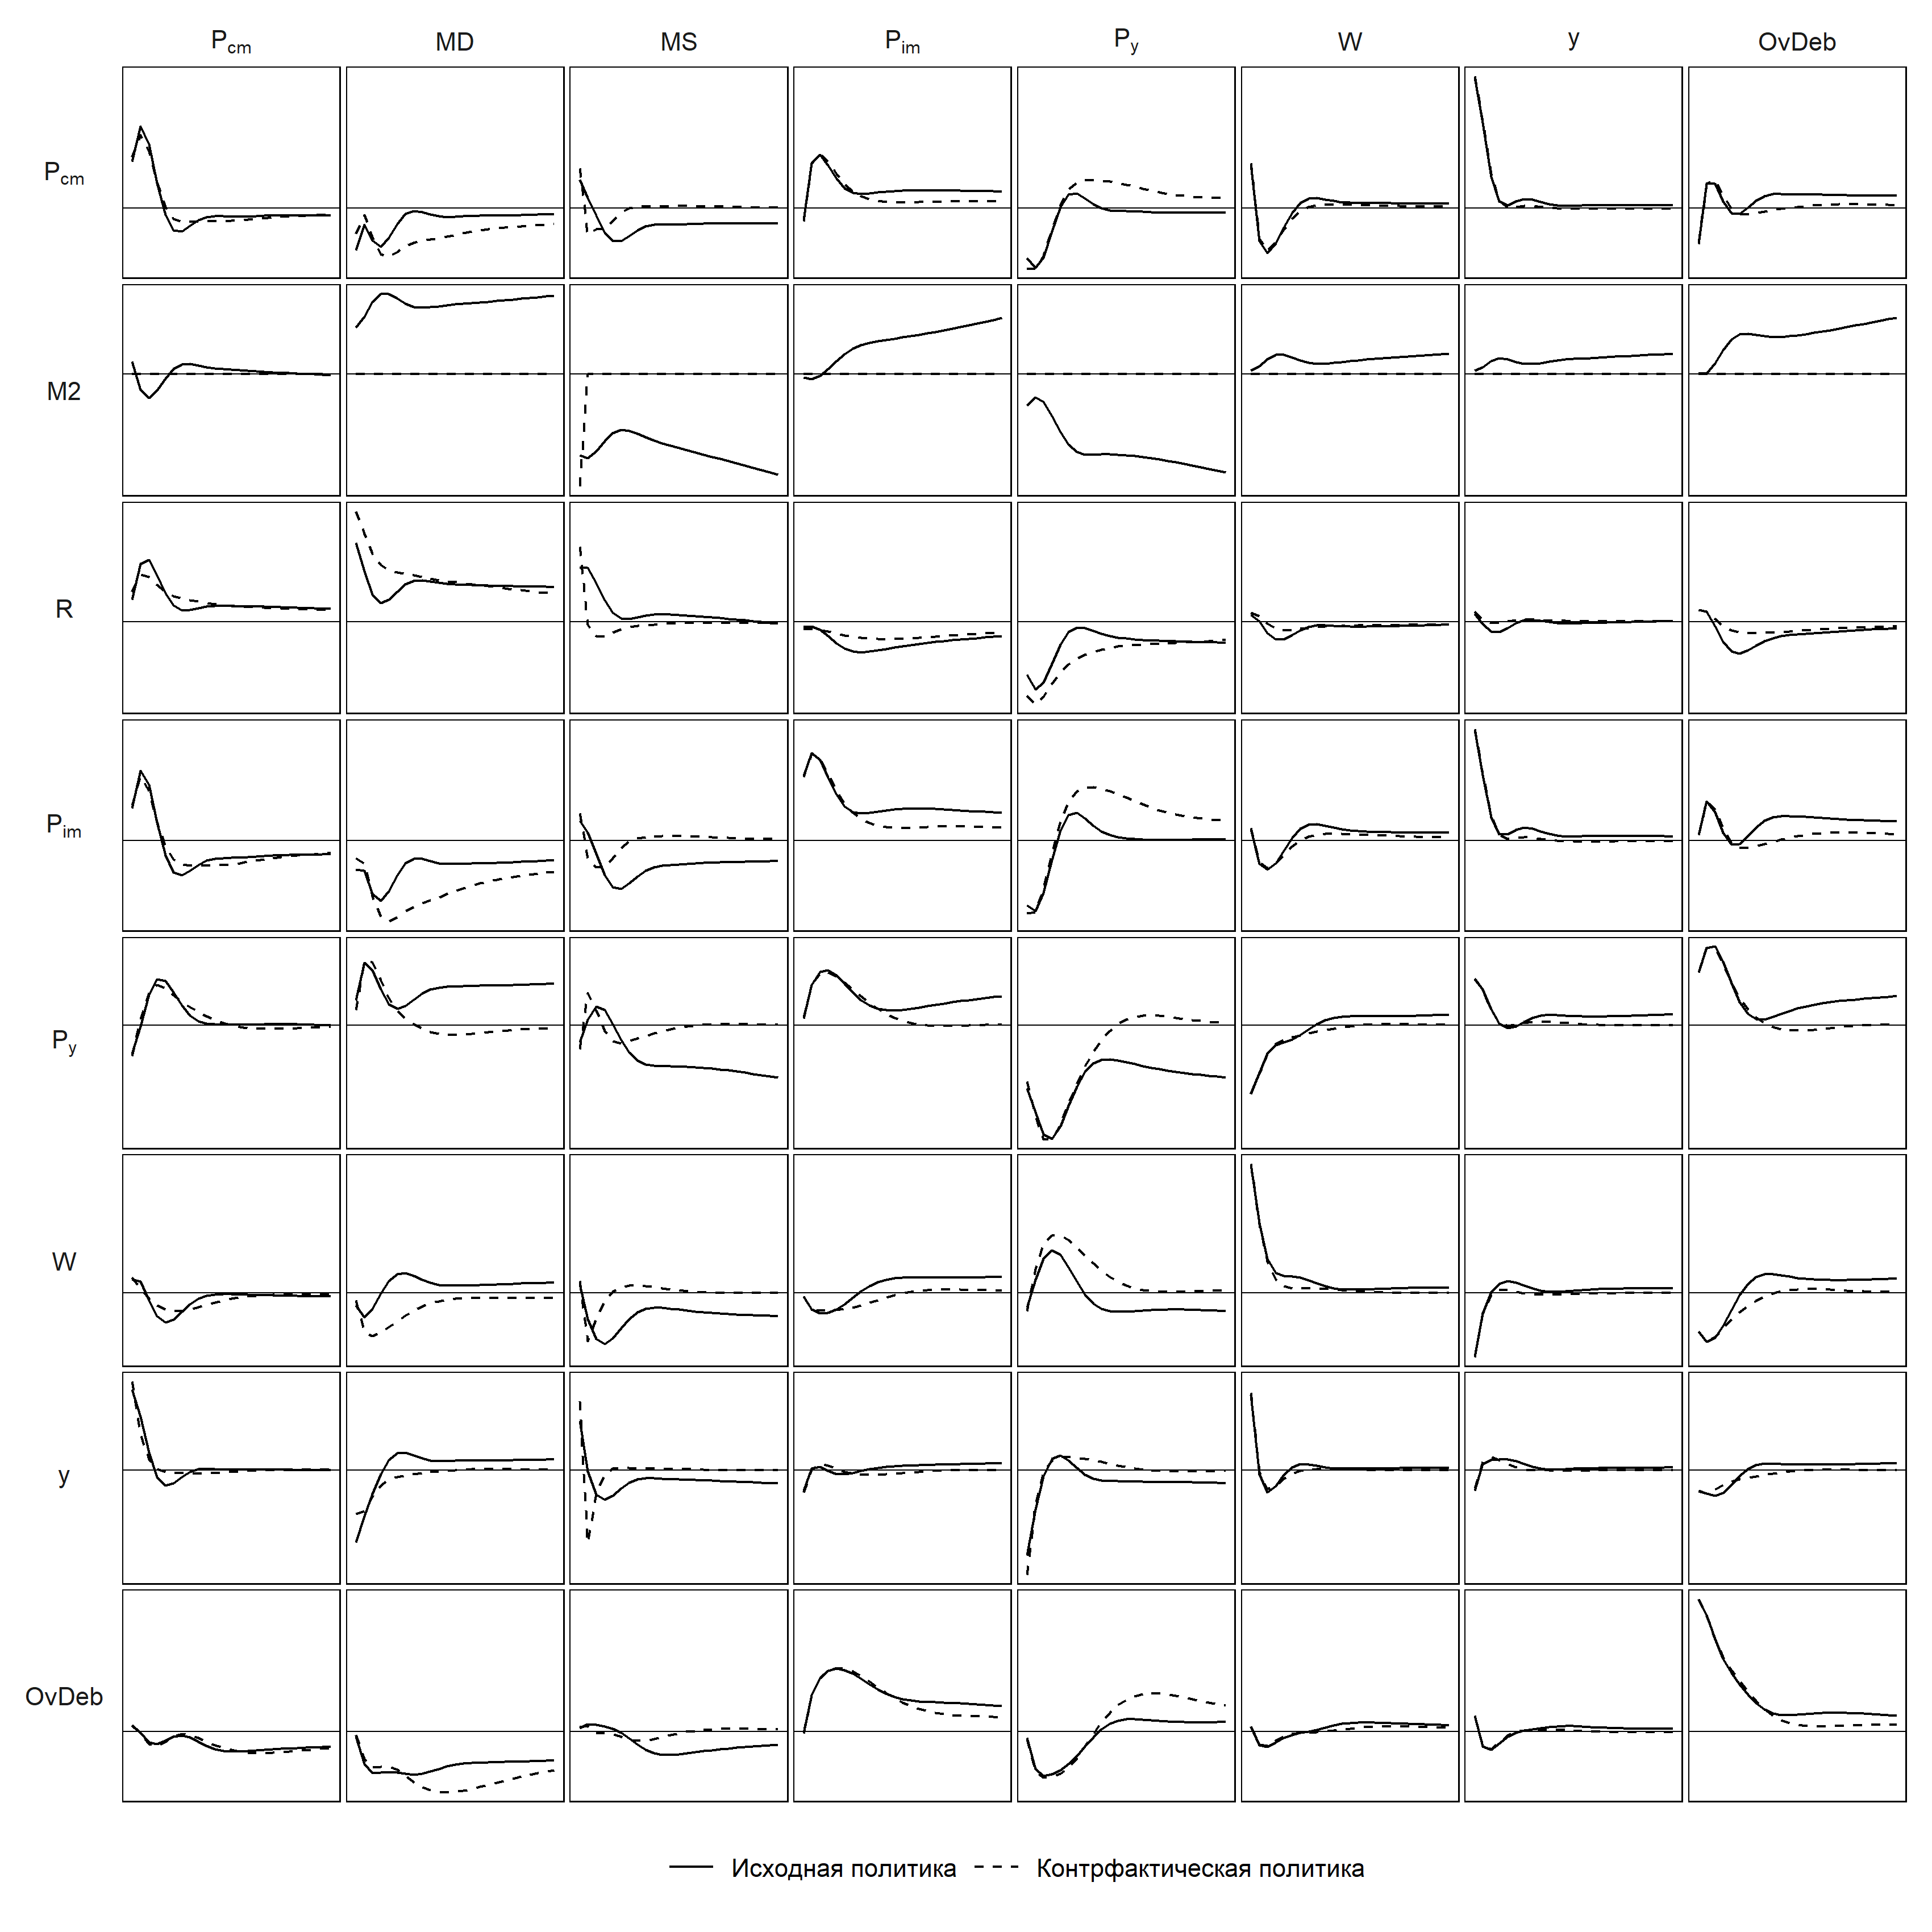
\includegraphics[width=\textwidth]{figures/output/policy_fixed_m2.png}
    \caption{Контрфактическая политика с фиксированным $M2$}
    \label{fig:policy-fixed-m2}
\end{figure}

\begin{figure}[!htbp]
    \centering
    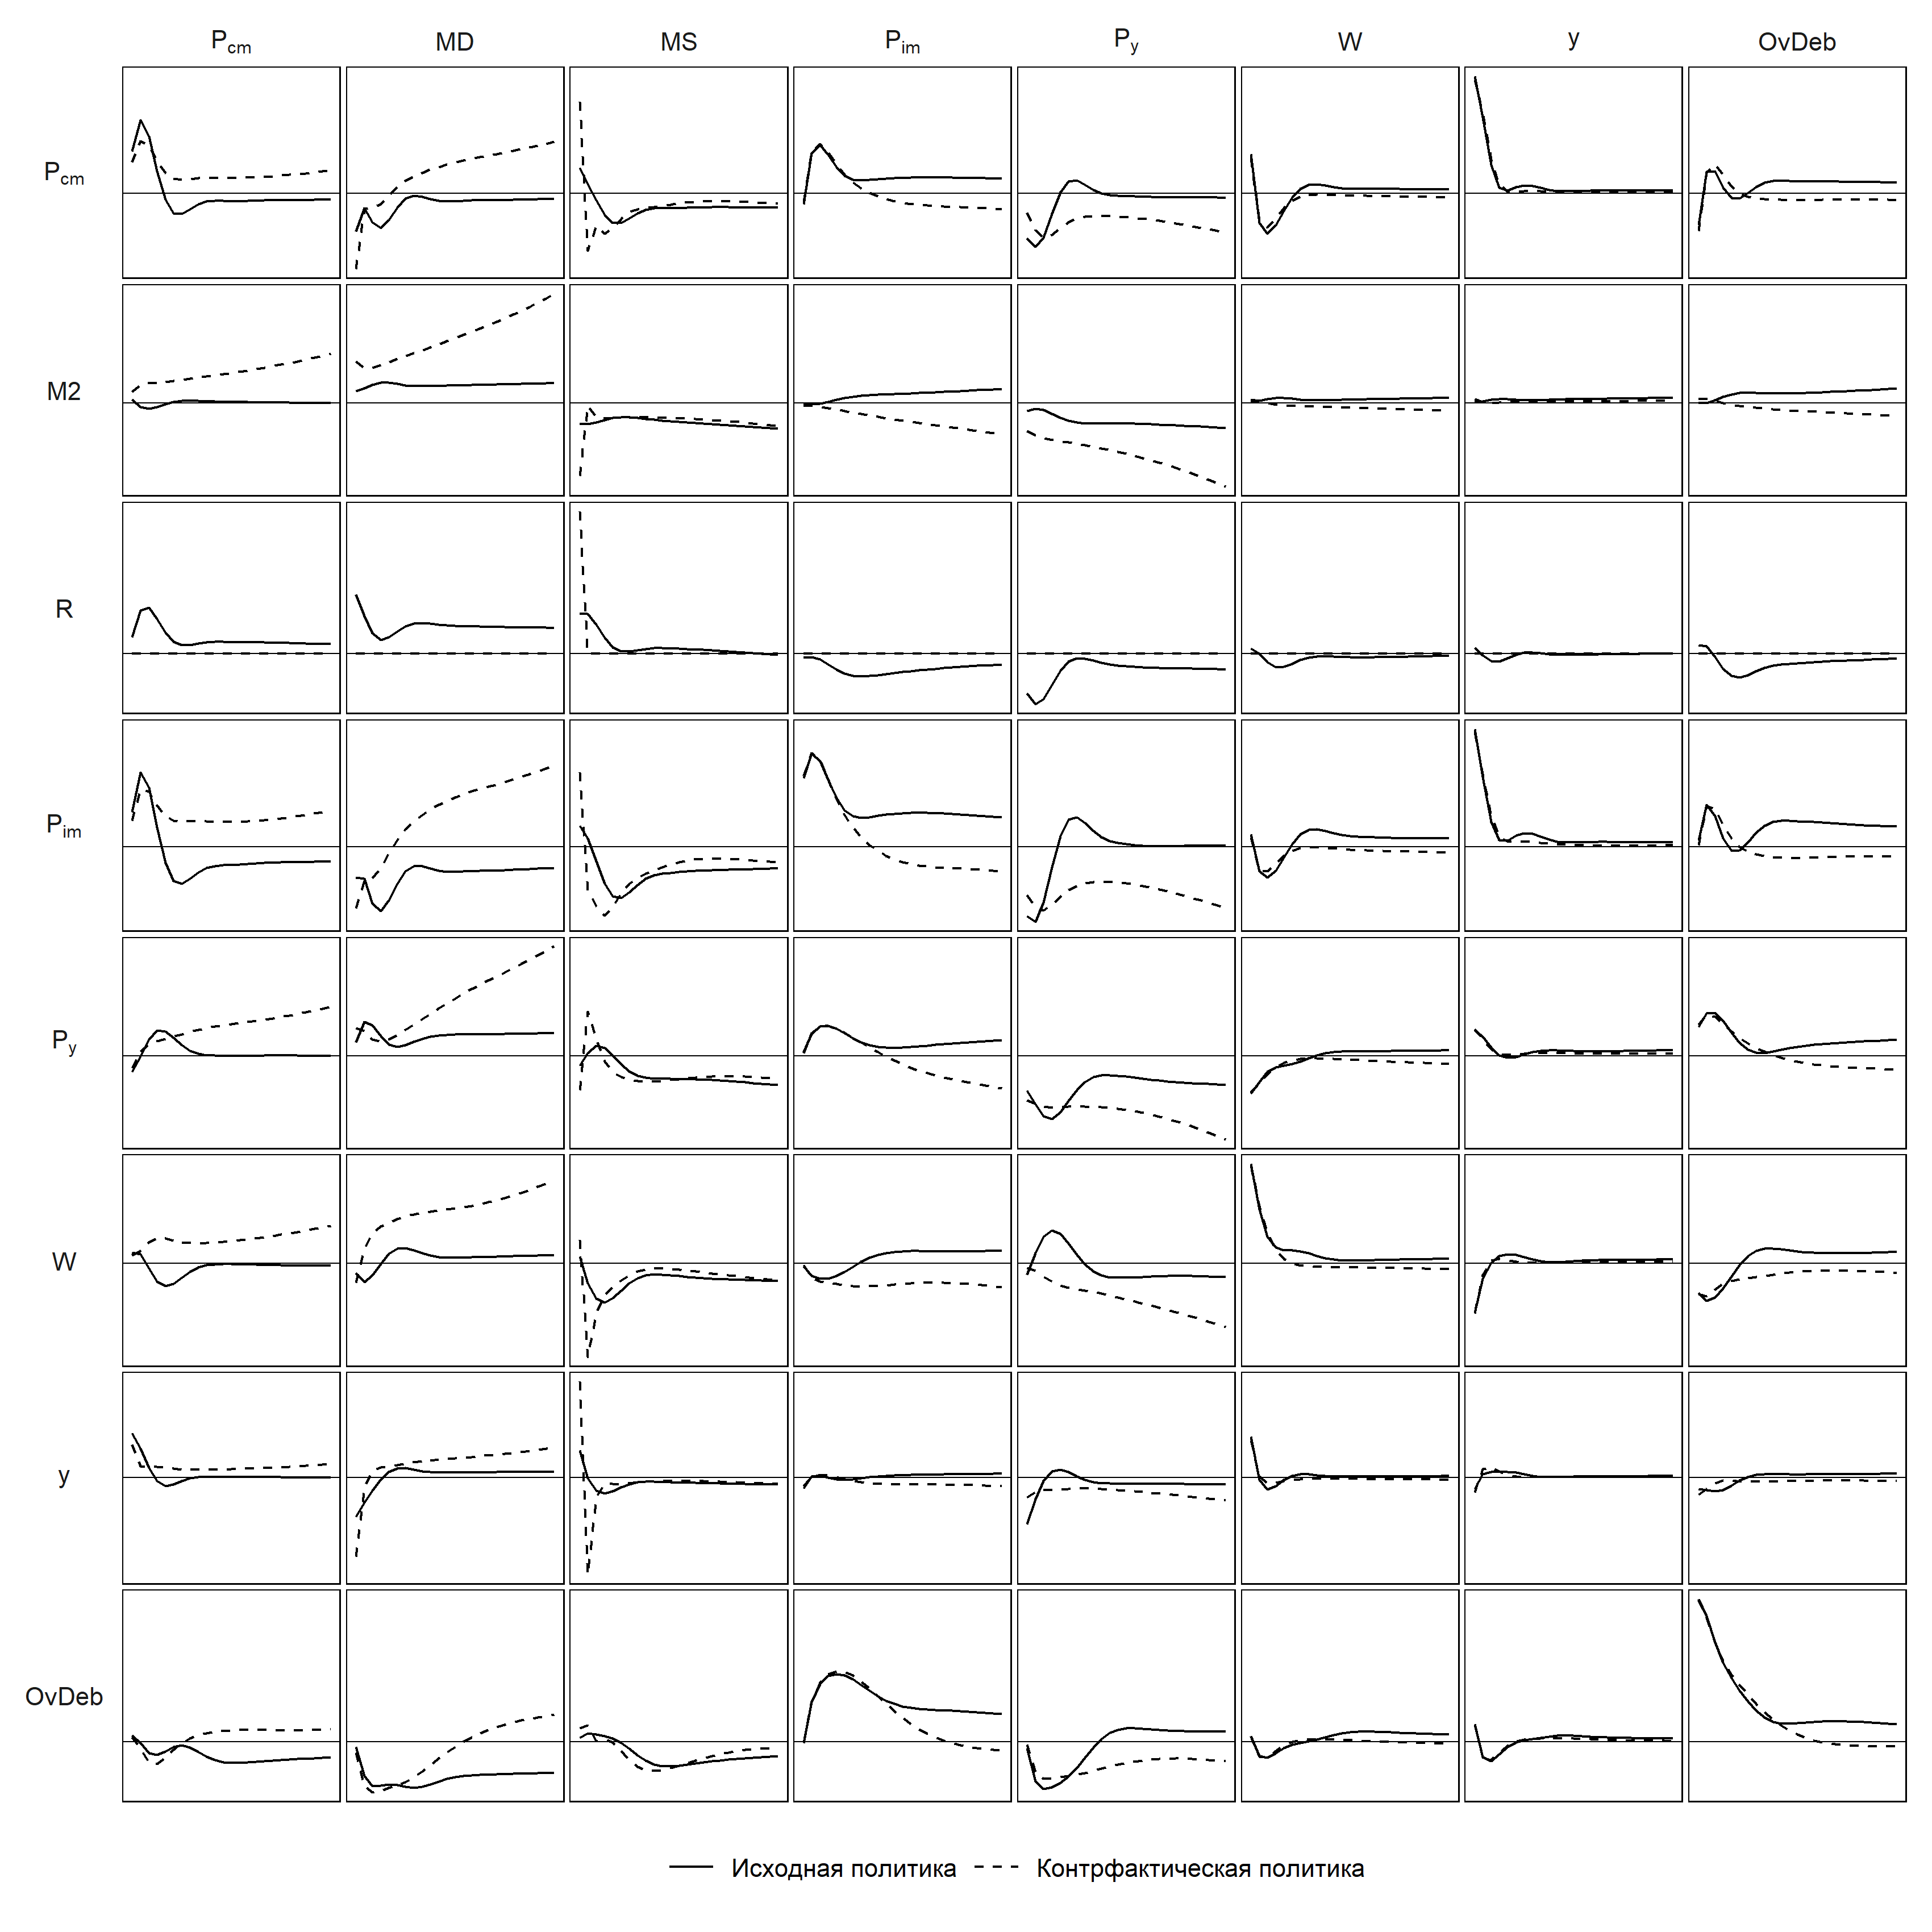
\includegraphics[width=\textwidth]{figures/output/policy_fixed_key_rate.png}
    \caption{Контрфактическая политика с фиксированной процентной ставкой $R$}
    \label{fig:policy-fixed-key-rate}
\end{figure}
На рисунках \ref{fig:policy-fixed-m2}--\ref{fig:policy-fixed-key-rate} сравниваются исходная политика и два контрфактических режима: фиксированный $M2$ и фиксированная ставка $R$. Сплошные линии показывают отклики в исходной модели, пунктирные --- отклики при изменённом правиле.

Как и в Sims и Zha, основной интерес связан не со столбцом $MS$, а с реакциями на неденежные шоки. При фиксированном $M2$ часть колебаний выпуска становится слабее, но реакции ценовых переменных иногда затухают медленнее. Поэтому такой режим не выглядит однозначно более стабилизирующим.

При фиксированной ставке $R$ различия заметнее. Модель ограничивает реакцию ставки, но часть шоков сильнее передаётся в $M2$, цены и выпуск. Это не устраняет нестабильность, а перераспределяет её между переменными.

В целом графики поддерживают вывод исторической декомпозиции: денежно-кредитная политика в модели не сводится к автономным шокам $MS$ и играет стабилизирующую роль при неденежных шоках. Простая фиксация $M2$ или $R$ не даёт очевидного улучшения относительно исходного правила.